\documentclass[a4paper]{article}
% Import some useful packages
\usepackage[margin=0.5in]{geometry} % narrow margins
\usepackage[utf8]{inputenc}
\usepackage[english]{babel}
\usepackage{hyperref}
\usepackage{bm}
\usepackage{listings}
\usepackage{amsmath,graphicx,varioref,verbatim,amsfonts,geometry,amssymb,dsfont,blindtext,wasysym}
%\usepackage{minted}
\usepackage{amsmath}
\usepackage{xcolor}
%\usepackage{minipage}
\usepackage{caption}

\usepackage{placeins}
\let\Oldsection\section
\renewcommand{\section}{\FloatBarrier\Oldsection}
\let\Oldsubsection\subsection
\renewcommand{\subsection}{\FloatBarrier\Oldsubsection}
\let\Oldsubsubsection\subsubsection
\renewcommand{\subsubsection}{\FloatBarrier\Oldsubsubsection}
\hypersetup{colorlinks=true}
\definecolor{LightGray}{gray}{0.95}
\definecolor{dkgreen}{rgb}{0,0.6,0}
\definecolor{gray}{rgb}{0.5,0.5,0.5}
\definecolor{mauve}{rgb}{0.58,0,0.82}
\definecolor{mygray}{rgb}{0.9,0.9,0.9}
\definecolor{LightGray}{gray}{0.95}
\lstset{frame=tb,
	language=Python,
	aboveskip=3mm,
	belowskip=3mm,
	showstringspaces=false,
	columns=flexible,
	basicstyle={\small\ttfamily},
	numbers=none,
	numberstyle=\tiny\color{gray},
	keywordstyle=\color{blue},
	commentstyle=\color{dkgreen},
	stringstyle=\color{mauve},
	backgroundcolor=\color{mygray}
	%breaklines=true,
	%breakatwhitespace=true,
	%tabsize=3
}

\usepackage{enumitem}
\setlistdepth{20}
\renewlist{itemize}{itemize}{20}
\setlist[itemize]{label=$\cdot$}

\title{Project 5 in FYS3150}
\author{Bendik Steinsvåg Dalen, Ulrik Seip}
%\renewcommand\thesection.\alph{section}
%\renewcommand\thesection{\Alph{section}}
\renewcommand\thesubsection{\thesection.\alph{subsection}}
\renewcommand\thesubsubsection{\thesubsection.\roman{subsubsection}}
\begin{document}
\maketitle


\begin{abstract}
	Stuff
\end{abstract}


\section{INTRODUCTION}


\section{METHOD}

\subsection{The SIRS method}

In the SIRS model we observe an isolated population of $N$ people which are divided into three separate groups:

\begin{itemize}
	\item $S$ for susceptible individuals, people who can become infected from the disease,
	\item $I$ for infected individuals, people who currently have the disease,
	\item $R$ for recovered individuals, people who no longer are sick and currently are immune to the disease.
\end{itemize}
The total population $N = S(t) + I(t) + R(t)$ will at least for now remain constant. An individual can move from $S$ to $I$, from $I$ to $R$, and from $R$ to $S$. The rate at which they do this will be referred to as $a$, $b$ and $c$ respectively. When an susceptible individual is in contact with an infected individual there is a chance that they become infected, while the rate of recovery and the rate of immunity loss is independent from the other groups. This can then be written as three coupled differential equations:
\begin{align}
S ^ { \prime } & = c R - \frac { a S I } { N } \\
I ^ { \prime } & = \frac { a S I } { N } - b I \\
R ^ { \prime } & = b I - c R \label{SIRS}
\end{align}

This set does not have a analytical solution, but we can easily study the equilibrium solutions. By setting \ref{SIRS} to 0 we get 
\begin{align} 
s ^ { * } & = \frac { b } { a }, \\ 
i ^ { * } & = \frac { 1 - \frac { b } { a } } { 1 + \frac { b } { c } }, \\ 
r ^ { * } & = \frac { b } { c } \frac { 1 - \frac { b } { a } } { 1 +  \frac{b}{c} }, \label{SIRS_eq}
\end{align}
where $s$, $i$ and $r$ denotes the fraction of people in $S$, $I$ and $R$, respectively, and $^*$ means that they are at equilibrium. These should add up to 1, and be between 0 and 1. 
One thing we can denote from this is that we need $b < a$ for the disease to establish itself in the population. However if $b>a$ the model brakes, as $s^*$ becomes larger than 1, and $i^*$ and $r^*$ becomes less than zero. This makes sense, as this would make the rate of recovery larger than the rate of infection, and the disease wouldn't be able to spread. 
These will serve as a good comparison for our numerical approximations. 


\subsection{Runge Kutta}
To solve equation \ref{SIRS} we will first be using the 4th. order Runge Kutta method. This is a pretty standar method for solving differntial equations. One cycle of the method is
\begin{align}
k_1 &= f(t_n,y_n) \\
k_2 &= f(t_n + \frac{\Delta t}{2},y_n + \frac{\Delta t}{2} k_1) \\
k_3 &= f(t_n + \frac{\Delta t}{2},y_n + \frac{\Delta t}{2} k_2) \\
k_4 &= f(t_n + \Delta t, y_n + \Delta t k_3) \\
y_{n+1} &= y_n + \frac{\Delta t}{6} \left( k_1 + 2k_2 + 2k_3 + k_4 \right),
\end{align}
where $y_n$ is the current step, $y_{n+1}$ is the next step, $t_n$ is the current time, $\Delta t$ is the timestep, and $f$ is the differntial equation. 
One problem ...

We will be observing four different populations $A$, $B$, $C$ and $D$. All of them are of size $N = 400$, and we start with 300 susceptible individuals and 100 infected individuals. We also set $a=4$ and $c=0.5$, but $b$ will vary from 1 to 4. We will set $\Delta t = 0.01 days$ and run the simulation until the equilibrium situation has been reached. 

We will also study a population $E$ where we set $b=5$ to se how this affects the situation. 


\subsection{Monte Carlo}

\subsection{Improving the modell}

Now that we have a basic modell we can extended it to include more details about the population and disease. Following are three different methods (?) that can improve the modell to make it more realistic. (We are going to implemet them independently at first, but then we are going to attempt to include all of them at the same time).

\subsubsection{Vital dynamics}

First we are going to include vital dynamics, meaning death and birth rate. This can be usefull if we are going to modell a population over a longer time period. We let $e$ be birth rate, $d$ be death rate and $d_i$ be the death rate from the disease. We assume that individuals from all the groups can give brith, but that children born into the population are initially susceptible. This makes differential equations into 
\begin{align} 
S ^ { \prime } & = c R - \frac { a S I } { N } - d S + e N, \\ 
I ^ { \prime } & = \frac { a S I } { N } - b I - d I - d _ { I } I, \\ 
R ^ { \prime } & = b I - c R - d R.
\end{align}

We tried to base the values for $d$ and $e$ on the death and birth rate in Norway. From (kilde) we find that these become $d=0.00002242299$ and $e=0.00002948891$ per day. We applied these to the populations $A$, $B$, $C$ and $D$, and observed how these were affected by setting $d_i=0$ and $d_i=0.1$. We then tried different values for $d_i$ on population $A$ to see if these would result in the entire population dying. Finally, as the values of $d$ and $e$ we found are quite low, we tried seeing how population $B$ would be affected by increasing these by a factor of 1000, 2000 and 10000. 


\subsubsection{Seasonal Variation}

Another concept we can study is seasonal variations in the infection rate. Certian diseases, such as influenza, have a large variance in infection rate based on the time of year. This can be modeled by setting $a$ to be
\begin{align}
a ( t ) = A \sin ( \omega t ) + a _ { 0 },
\end{align}
where $a0$ is the average transmission rate, $A$ is the maximum deviation from $a_0$, and $\omega$ is the frequency of oscillation. We set $\omega = 2 \pi/365.25$ so that $a$ would have a variance of a year, like most diseases. Fist we set $A=1$ and $a0=4$ for population $A$ and $D$. Then we observed population $B$, and set $A=2$, and $a0=4$ and $6$. 


\subsubsection{Vaccination}

For many diseases a vaccine gets developed. A vaccine causes an susceptible individual to become immune, effectively moving them to the recovered group. We assume that the rate of vaccination $f$ is independent from how many people already have been vaccinated, but that it can vary with time. We also assume that vaccinated individuals loose their immunity at the same rate as people who have recovered from the disease. The differential equations then becomes
\begin{align} 
S ^ { \prime } & = c R - \frac { a S I } { N } - d S -f, \\ 
I ^ { \prime } & = \frac { a S I } { N } - b I , \\ 
R ^ { \prime } & = b I - c R + f.
\end{align}

Exactly what $f$ is can vary. We will be studing three cases:
\begin{itemize}
	\item Constant $f$, meaning $f = f_c S$, where $f_c$ is some constant. We sat $f_c = 1$ for population $A$, $B$, $C$ and $D$. For some diseases a vaccine is offered to children at a specific age, which would constitute a constant vaccination rate. However, these vaccines usally induce a permanent or a long lasting immunity, so this method migth not fit well with our modell.
	\item Linear $f$, meaning $f = (t \cdot f_l + f_0) \cdot I$, where $f_0$ is the initial value of $f$, and $f_l$ is the rate at which $f$ increases with time. We sat $f_0 = 0$ and $f_l = 0.01$ for population $A$, $B$, $C$ and $D$. 
	This is meant to modell that as awareness and medical research increases, more people take the vaccine and the vaccine becomes more effective. If having this increase linearly is the most realistic way is unknown, but we assume it's a good approximation. By setting $f_0 = 0$ we start the simmualtion at the point when vaccination starts.
	\item Vaccination campaign $f$. This method is meant to modell a how many governments respond to an outbreak of an epidemic, by distributing vaccines during a certian time period, often called an vaccination campaign. This can be written as $f = f_c S$ if $t \in [t_0,t_1]$ and $f = f_n S$ if $t \notin [t_0,t_1]$, where $f_c >> f_n$. We sat $f_n=0$, $f_c=0.3$, $t_0=2$ and $t_1=9$ for population $A$, $B$, $C$ and $D$. 
\end{itemize}

\subsection{more monte carlo}

\section{RESULTS}

\subsection{The SIRS method}

\subsection{RungeKutta}

The resulting plots for population $A$ to $E$ can be seen in figure \ref{fig:opp_a_A} to \ref{fig:opp_a_E}. The resulting end values can alos be seen in table \ref{tab:opp_a_A} to \ref{tab:opp_a_E}.

\begin{figure}
	\centering
	\begin{minipage}{0.49\textwidth}
		\centering
		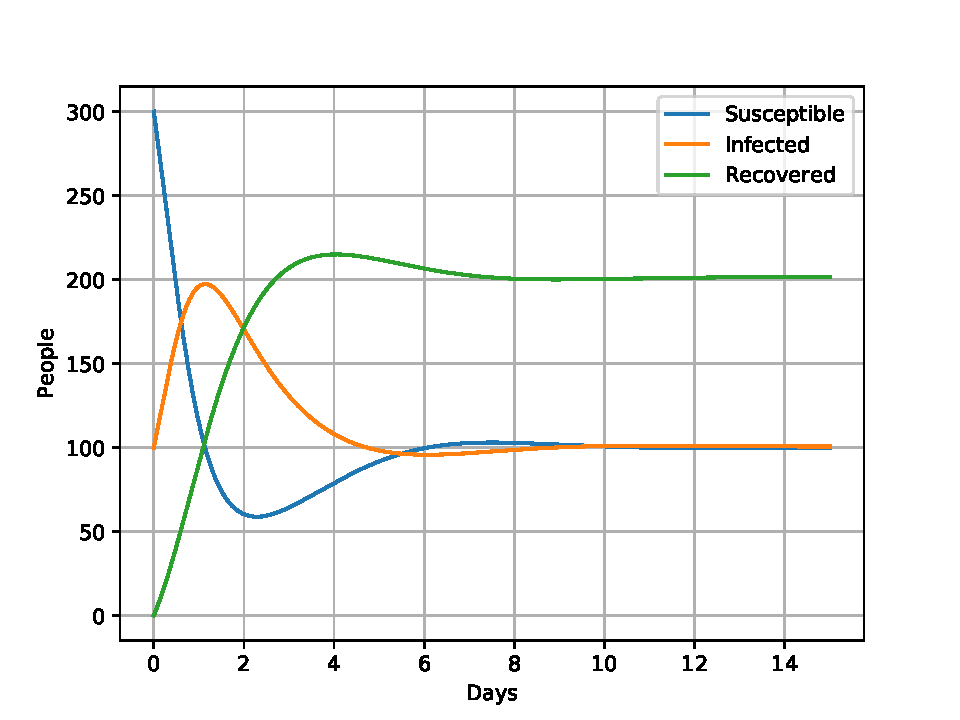
\includegraphics[scale=0.6]{../plots/opp_a_A.pdf}
		\caption{A plot of the population distribution for the SIRS-modell, for population $A$, where $a=4$, $b=1$ and $c=0.5$. }\label{fig:opp_a_A}
	\end{minipage}
	\begin{minipage}{0.49\textwidth}
		\centering
		\captionsetup{type=table} %% tell latex to change to table
		\begin{tabular}{|l|l|l|l|}
			\hline
			Group & Expected & Analytical   & Number  \\ \hline
			$s^*$ & 0.25 & 0.2499 & 100.0 \\ \hline
			$i^*$ & 0.25 & 0.2516 & 100.6 \\ \hline
			$r^*$ & 0.5  & 0.5035 & 201.4 \\ \hline
		\end{tabular}
		\caption{The corresponding end values for figure \ref{fig:opp_a_A}. The excpected values are derived from equation \ref{SIRS_eq}, the analytical values are the potion of the population found by RK4, and number are the total number  of people this corresponds to.}\label{tab:opp_a_A}
	\end{minipage}
%	\caption{stuff}
\end{figure}

\begin{figure}
	\centering
	\begin{minipage}{0.49\textwidth}
		\centering
		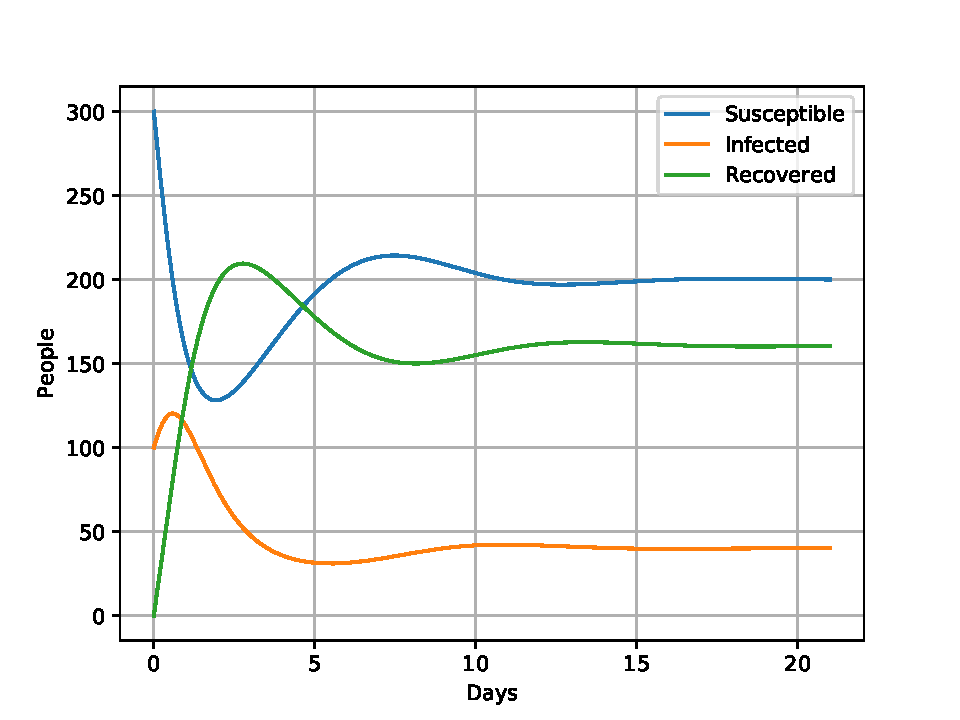
\includegraphics[scale=0.6]{../plots/opp_a_B.pdf}
		\caption{A plot of the population distribution for the SIRS-modell, for population $B$, where $a=4$, $b=2$ and $c=0.5$. }\label{fig:opp_a_B}
	\end{minipage}
	\begin{minipage}{0.49\textwidth}
		\centering
		\captionsetup{type=table} %% tell latex to change to table
		\begin{tabular}{|l|l|l|l|}
			\hline
			Group & Expected & Analytical   & Number  \\ \hline
			$s^*$ & 0.5 & 0.5001 & 200.1 \\ \hline
			$i^*$ & 0.1 & 0.1006 & 40.2 \\ \hline
			$r^*$ & 0.4 & 0.4011 & 160.5 \\ \hline
		\end{tabular}
		\caption{The corresponding end values for figure \ref{fig:opp_a_B}. The excpected values are derived from equation \ref{SIRS_eq}, the analytical values are the potion of the population found by RK4, and number are the total number  of people this corresponds to.}\label{tab:opp_a_B}
	\end{minipage}
	%	\caption{stuff}
\end{figure}

\begin{figure}
	\centering
	\begin{minipage}{0.49\textwidth}
		\centering
		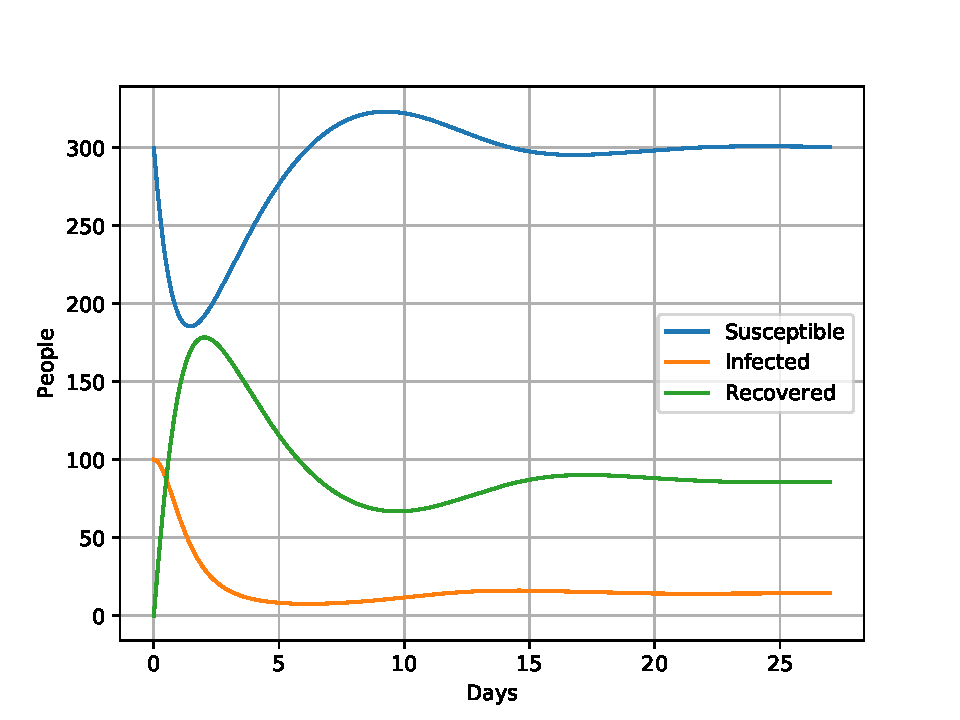
\includegraphics[scale=0.6]{../plots/opp_a_C.pdf}
		\caption{A plot of the population distribution for the SIRS-modell, for population $C$, where $a=4$, $b=3$ and $c=0.5$. }\label{fig:opp_a_C}
	\end{minipage}
	\begin{minipage}{0.49\textwidth}
		\centering
		\captionsetup{type=table} %% tell latex to change to table
		\begin{tabular}{|l|l|l|l|}
			\hline
			Group & Expected & Analytical   & Number  \\ \hline
			$s^*$ & 0.75 & 0.7511 & 300.5 \\ \hline
			$i^*$ & 0.0357 & 0.0360 & 14.4 \\ \hline
			$r^*$ & 0.2143 & 0.2145 & 85.8 \\ \hline
		\end{tabular}
		\caption{The corresponding end values for figure \ref{fig:opp_a_C}. The excpected values are derived from equation \ref{SIRS_eq}, the analytical values are the potion of the population found by RK4, and number are the total number  of people this corresponds to.}\label{tab:opp_a_C}
	\end{minipage}
	%	\caption{stuff}
\end{figure}

\begin{figure}
	\centering
	\begin{minipage}{0.49\textwidth}
		\centering
		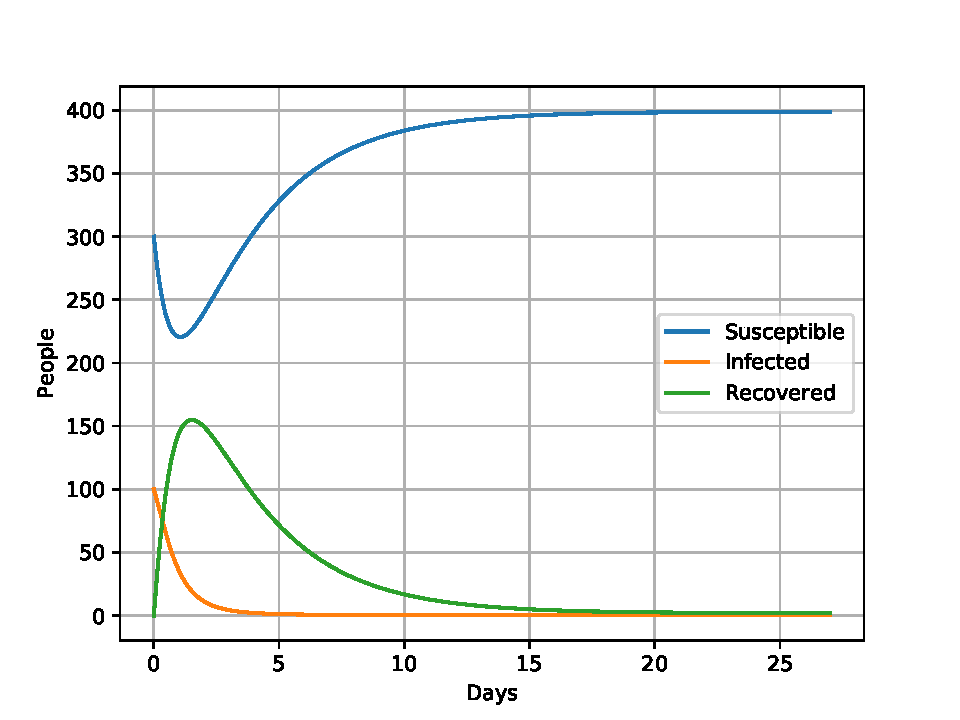
\includegraphics[scale=0.6]{../plots/opp_a_D.pdf}
		\caption{A plot of the population distribution for the SIRS-modell, for population $D$, where $a=4$, $b=4$ and $c=0.5$. }\label{fig:opp_a_D}
	\end{minipage}
	\begin{minipage}{0.49\textwidth}
		\centering
		\captionsetup{type=table} %% tell latex to change to table
		\begin{tabular}{|l|l|l|l|}
			\hline
			Group & Expected & Analytical   & Number  \\ \hline
			$s^*$ & 1.0 & 0.9974 & 399.0 \\ \hline
			$i^*$ & 0.0 & 0.0006 & 0.2 \\ \hline
			$r^*$ & 0.0 & 0.0047 & 1.9 \\ \hline
		\end{tabular}
		\caption{The corresponding end values for figure \ref{fig:opp_a_D}. The excpected values are derived from equation \ref{SIRS_eq}, the analytical values are the potion of the population found by RK4, and number are the total number  of people this corresponds to.}\label{tab:opp_a_D}
	\end{minipage}
	%	\caption{stuff}
\end{figure}

\begin{figure}
	\centering
	\begin{minipage}{0.49\textwidth}
		\centering
		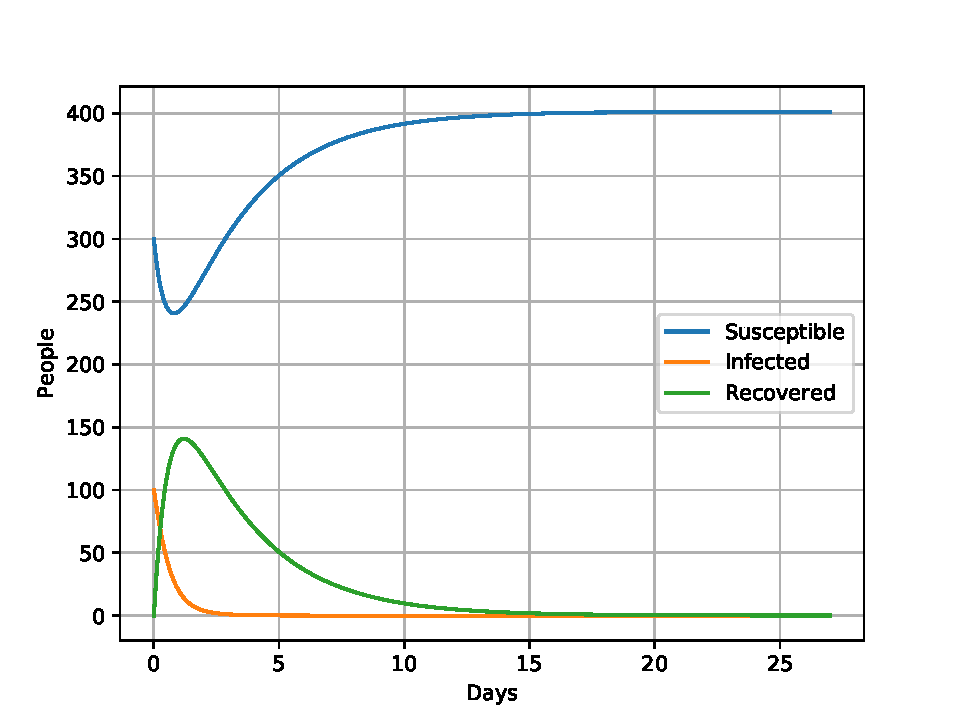
\includegraphics[scale=0.6]{../plots/opp_a_E.pdf}
		\caption{A plot of the population distribution for the SIRS-modell, for population $E$, where $a=4$, $b=5$ and $c=0.5$. }\label{fig:opp_a_E}
	\end{minipage}
	\begin{minipage}{0.49\textwidth}
		\centering
		\captionsetup{type=table} %% tell latex to change to table
		\begin{tabular}{|l|l|l|l|}
			\hline
			Group & Expected & Analytical   & Number  \\ \hline
			$s^*$ & 1.25 & 1.0034 & 401.4 \\ \hline
			$i^*$ & -0.0227 & $4.7119\cdot 10^{-11}$ & $1.9\cdot 10^{-8}$ \\ \hline
			$r^*$ & -0.2273 & $8.4064\cdot 10^{-5}$ & $3.4\cdot 10^{-2}$ \\ \hline
		\end{tabular}
		\caption{The corresponding end values for figure \ref{fig:opp_a_E}. The excpected values are derived from equation \ref{SIRS_eq}, the analytical values are the potion of the population found by RK4, and number are the total number  of people this corresponds to.}\label{tab:opp_a_E}
	\end{minipage}
	%	\caption{stuff}
\end{figure}


\subsection{Monte Carlo}

Stuff

\subsection{Vital dynamics}

\begin{figure}[!htb]
	\centering 
	%Scale angir størrelsen på bildet. Bildefilen må ligge i samme mappe som tex-filen. 
	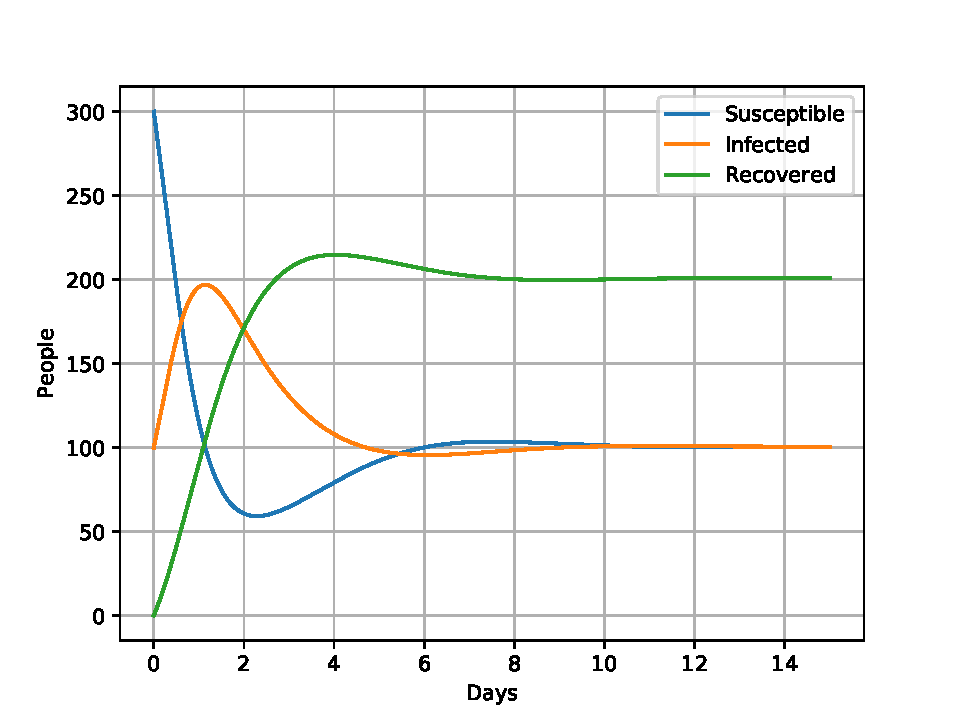
\includegraphics[scale=0.56]{../plots/opp_c_A0.pdf}
	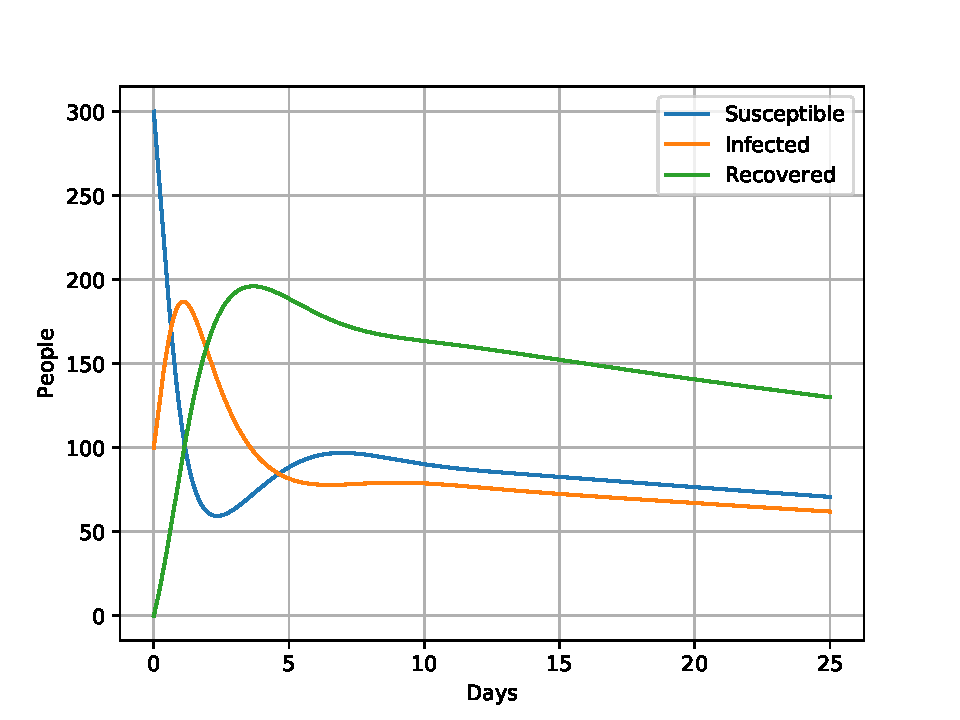
\includegraphics[scale=0.56]{../plots/opp_c_A1.pdf}
	\caption{Plots of population $A$ when accounting for vital dynamics. On the left $d_i=0$ and on the rigth $d_i=0.1$.}
	%Label gjør det enkelt å referere til ulike bilder.
	\label{opp_c0A}
\end{figure}
\begin{figure}[!htb]
	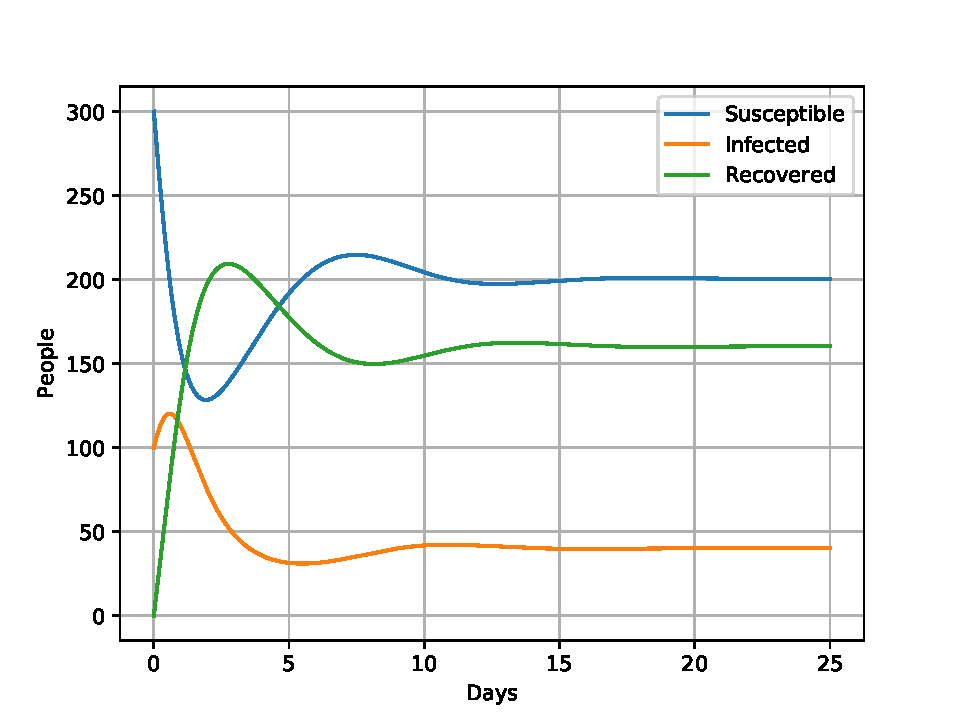
\includegraphics[scale=0.56]{../plots/opp_c_B0.pdf}
	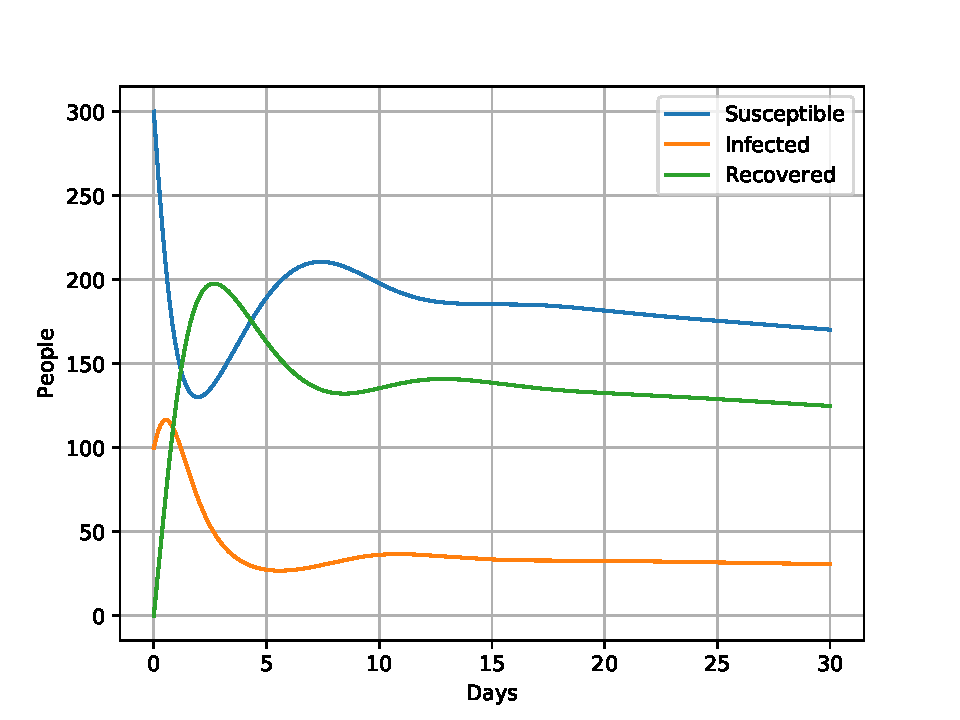
\includegraphics[scale=0.56]{../plots/opp_c_B1.pdf}
	\caption{Plots of population $B$ when accounting for vital dynamics. On the left $d_i=0$ and on the rigth $d_i=0.1$.}
	%Label gjør det enkelt å referere til ulike bilder.
	\label{opp_c0B}
\end{figure}	
\begin{figure}[!htb]
	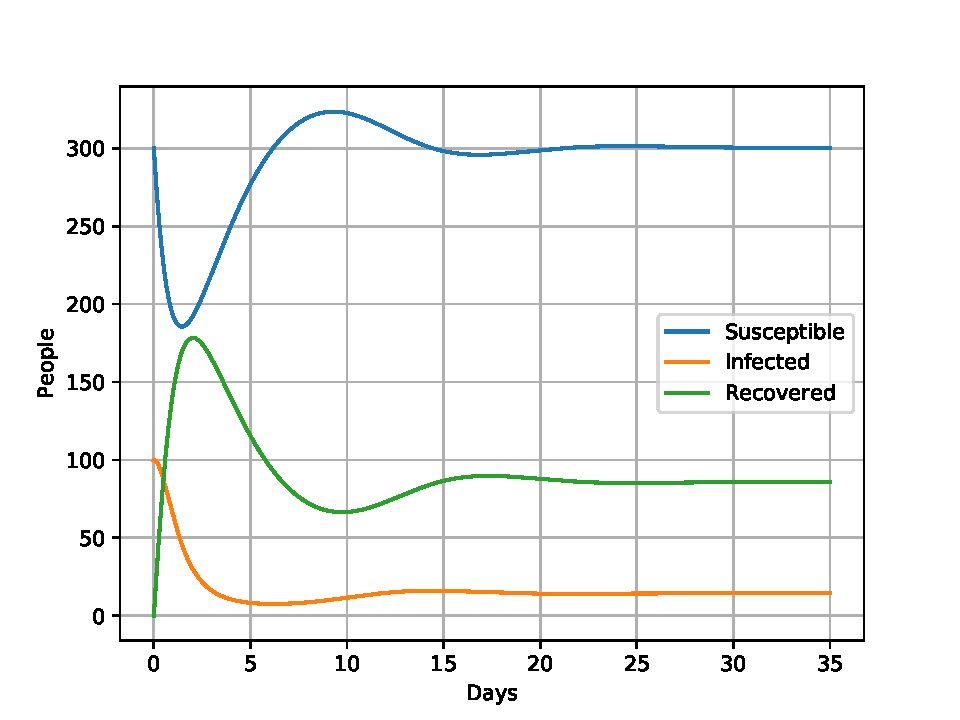
\includegraphics[scale=0.56]{../plots/opp_c_C0.pdf}
	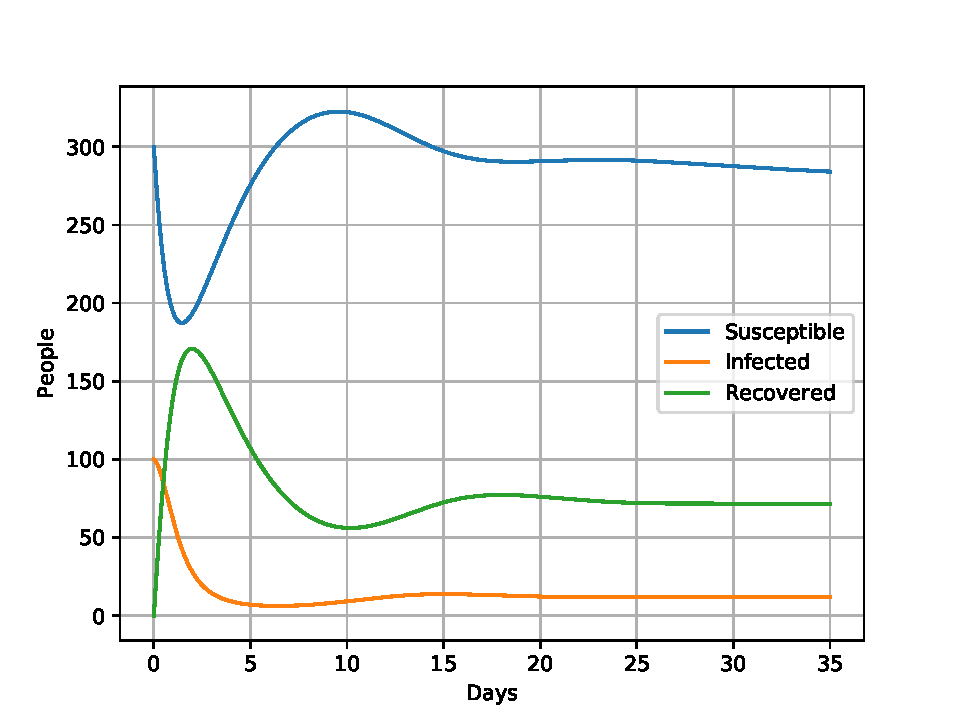
\includegraphics[scale=0.56]{../plots/opp_c_C1.pdf}
	\caption{Plots of population $C$ when accounting for vital dynamics. On the left $d_i=0$ and on the rigth $d_i=0.1$.}
	%Label gjør det enkelt å referere til ulike bilder.
	\label{opp_c0C}
\end{figure}
\begin{figure}[!htb]
	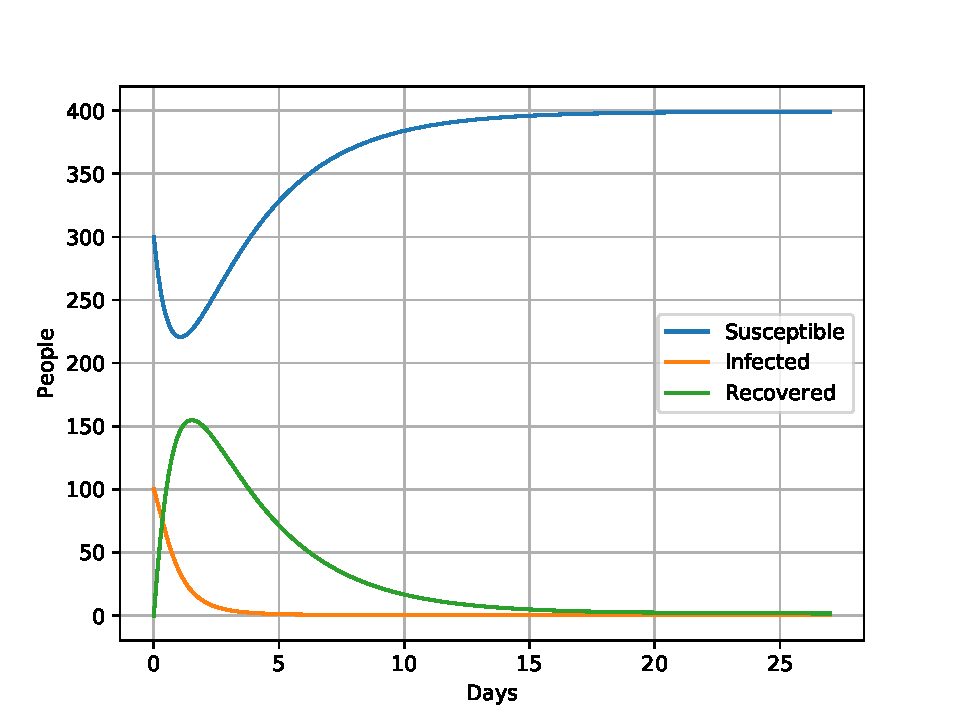
\includegraphics[scale=0.56]{../plots/opp_c_D0.pdf}
	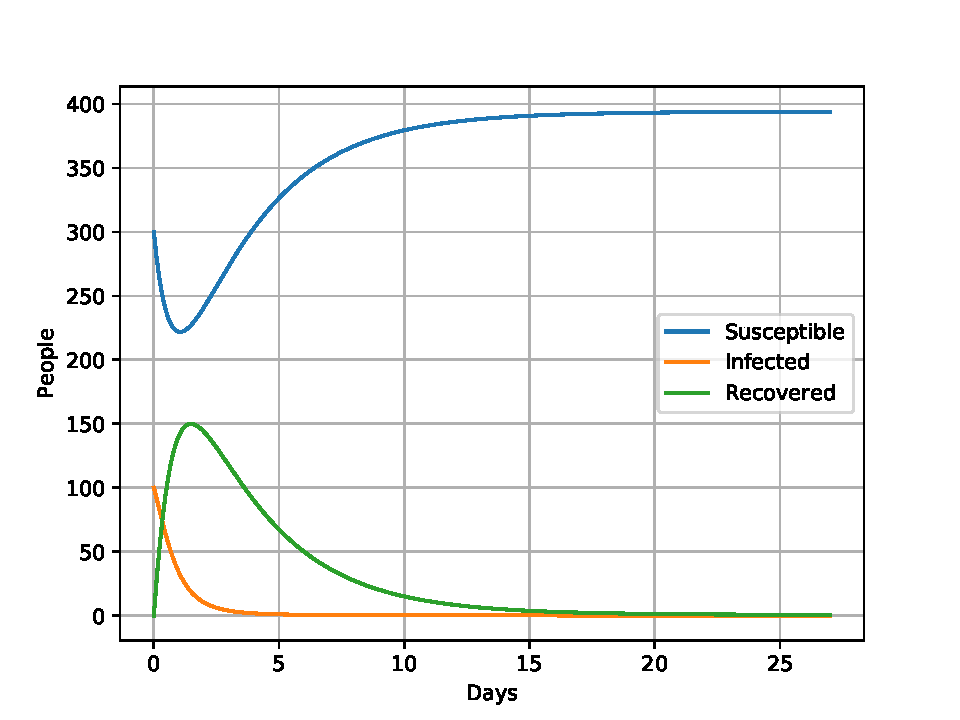
\includegraphics[scale=0.56]{../plots/opp_c_D1.pdf}	
	\caption{Plots of population $D$ when accounting for vital dynamics. On the left $d_i=0$ and on the rigth $d_i=0.1$.}
	%Label gjør det enkelt å referere til ulike bilder.
	\label{opp_c0D}
\end{figure}

\begin{figure}[!htb]
	\centering 
	%Scale angir størrelsen på bildet. Bildefilen må ligge i samme mappe som tex-filen. 
	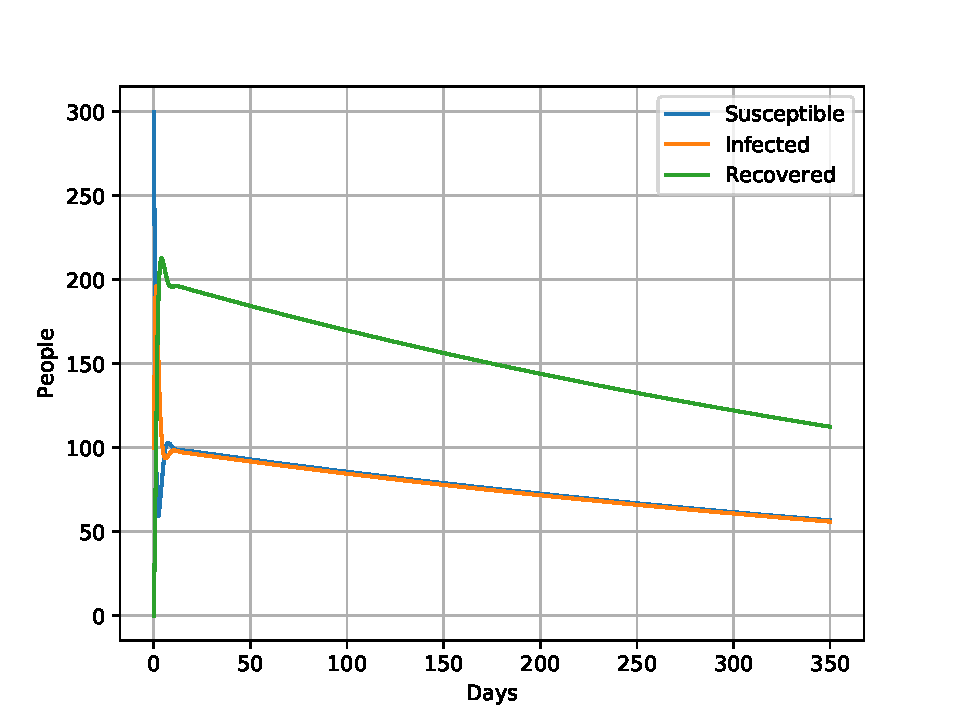
\includegraphics[scale=0.56]{../plots/opp_c_k3.pdf} %kan kaskje være først?
	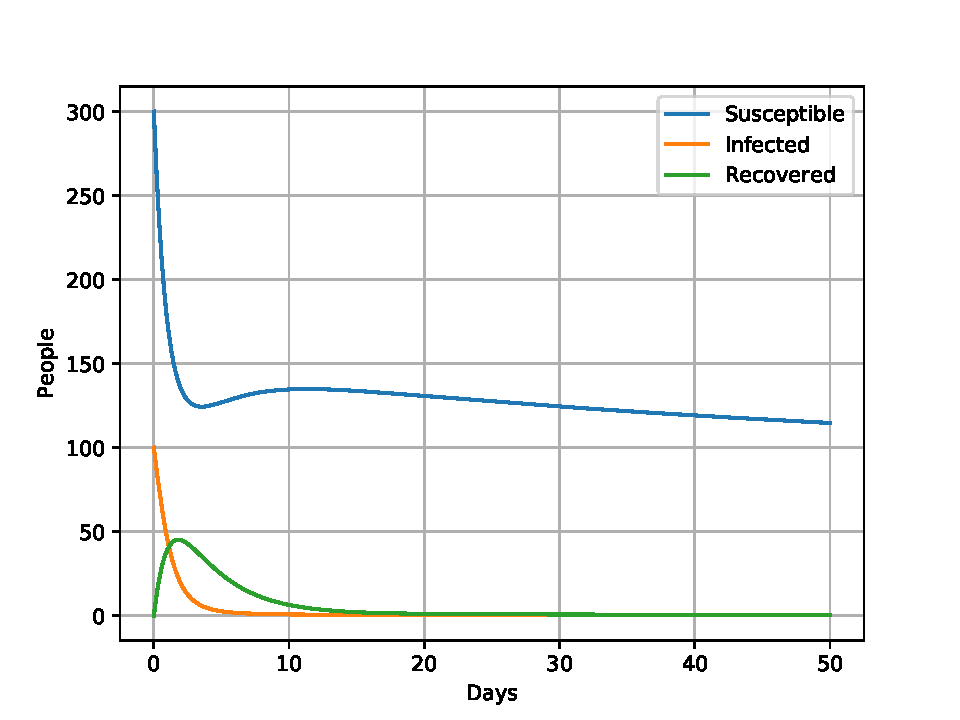
\includegraphics[scale=0.56]{../plots/opp_c_k0.pdf}
	\caption{Plots of population $A$ when accounting for vital dynamics. On the left $d_i=0.01$ and on the rigth $d_i=3$. The left $d_i$ is too low to effectively kill the entire population, while the one is too large.}
%	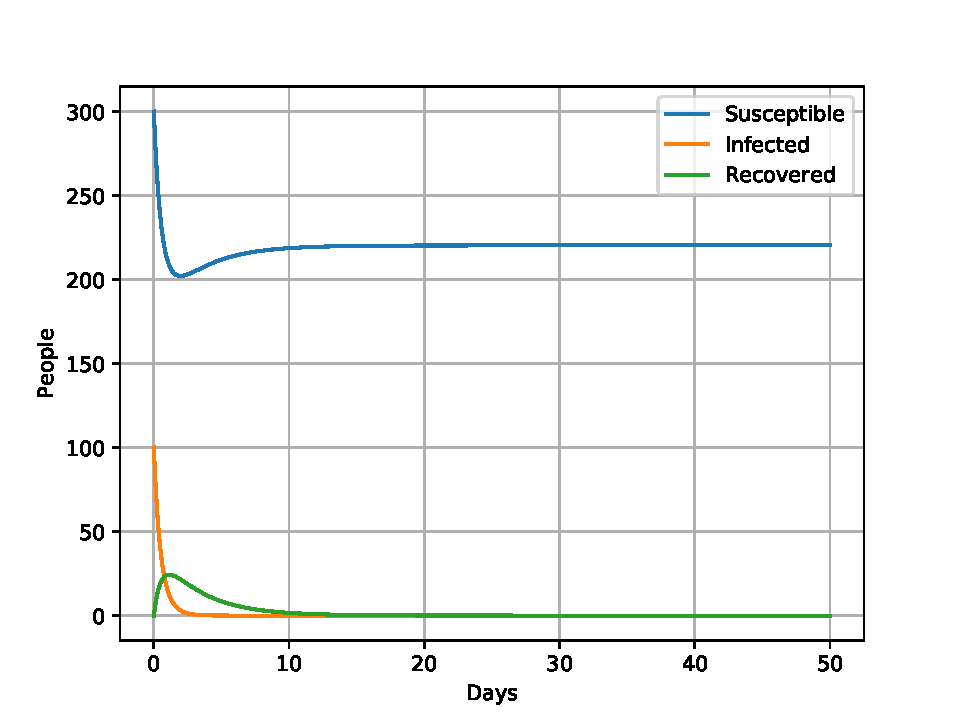
\includegraphics[scale=0.56]{../plots/opp_c_k1.pdf}
	%trenger kansjke ikke begge disse
%	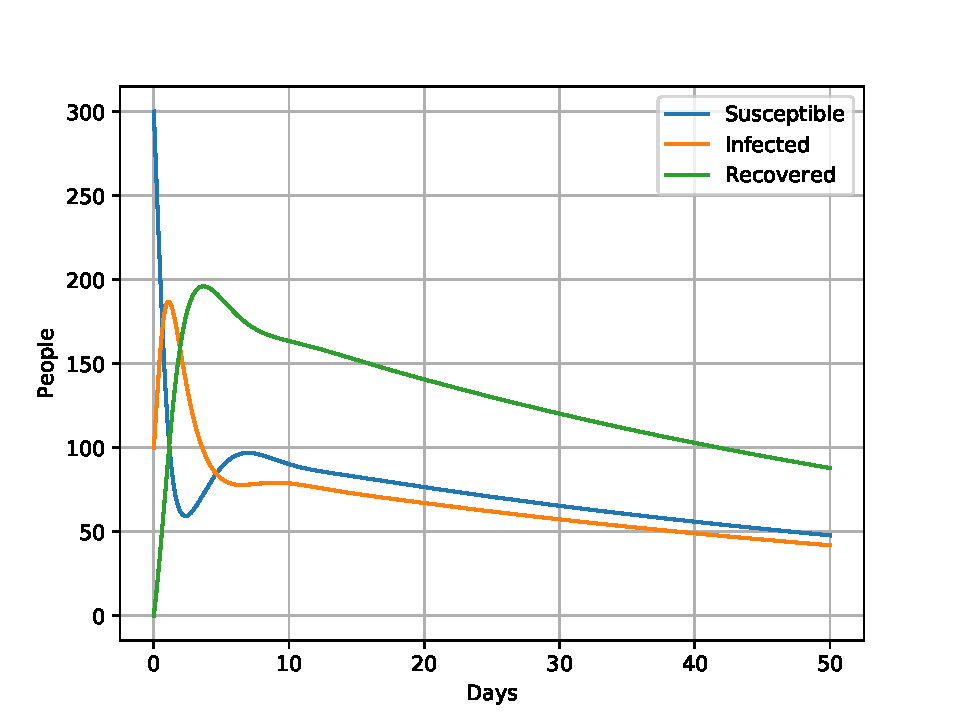
\includegraphics[scale=0.56]{../plots/opp_c_k2.pdf}
	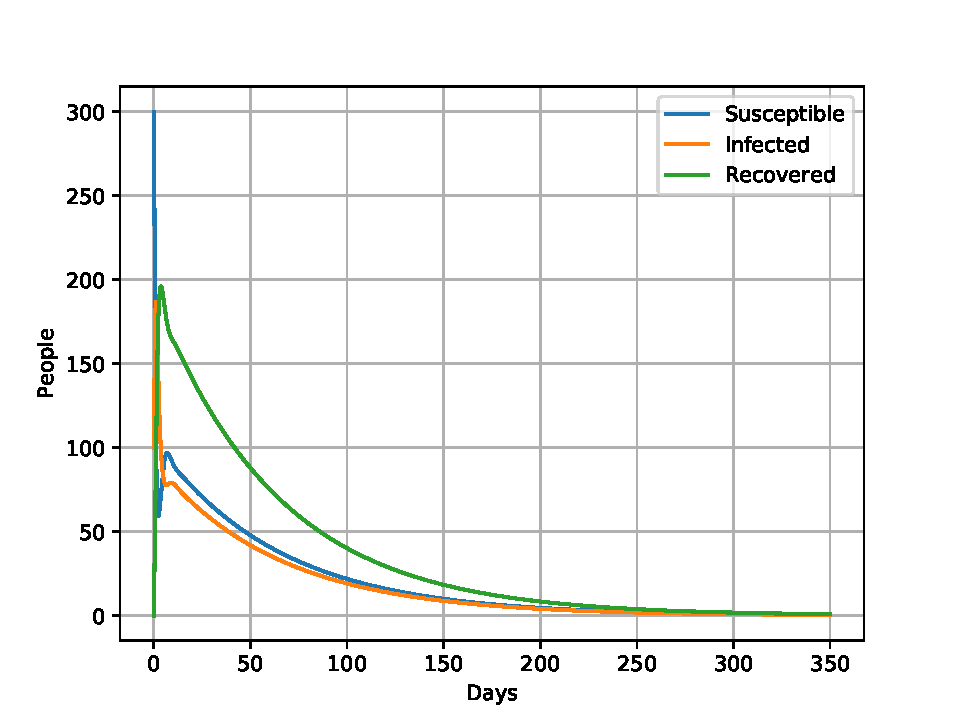
\includegraphics[scale=0.56]{../plots/opp_c_k2l.pdf}	
	%mulig jeg bør splitte denne
	\caption{Plots of population $A$ when accounting for vital dynamics with $d_i=0.1$. Here $d_i$ is the correct size to kill the entire population. }
	%Label gjør det enkelt å referere til ulike bilder.
	\label{opp_c1}
\end{figure}

\begin{figure}[!htb]
	\centering 
	%Scale angir størrelsen på bildet. Bildefilen må ligge i samme mappe som tex-filen. 
	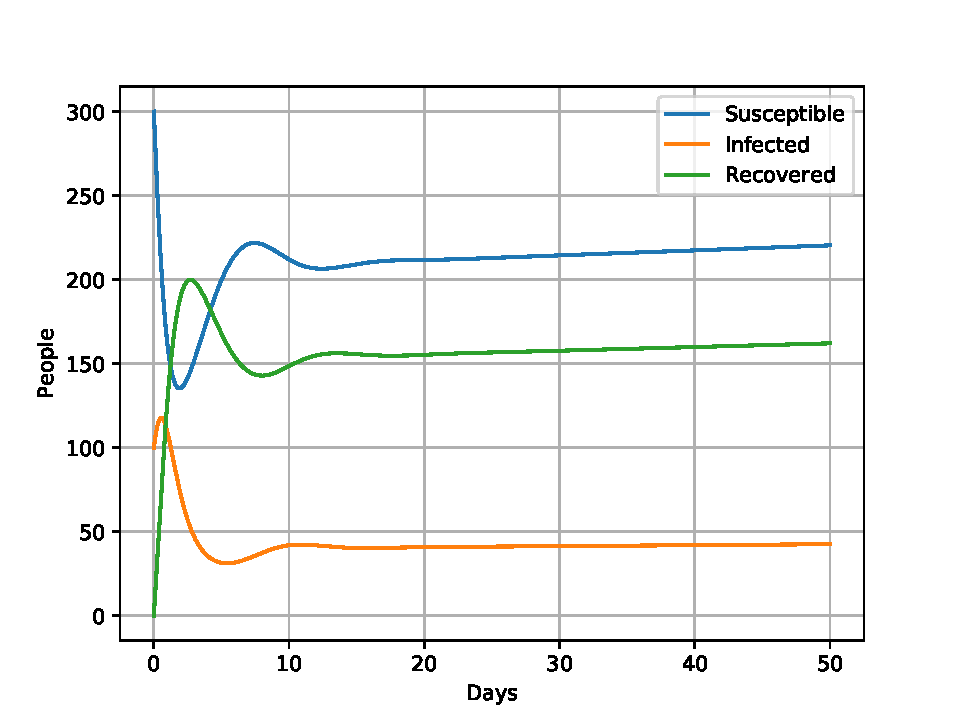
\includegraphics[scale=0.56]{../plots/opp_c_h_10000.pdf}
	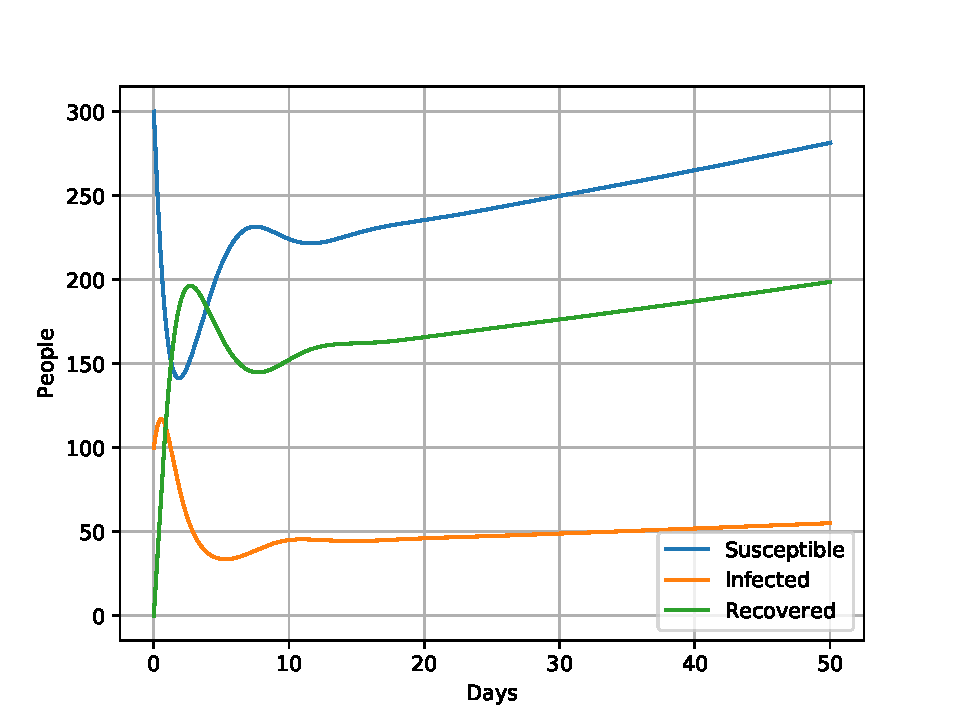
\includegraphics[scale=0.56]{../plots/opp_c_h_20000.pdf}	
	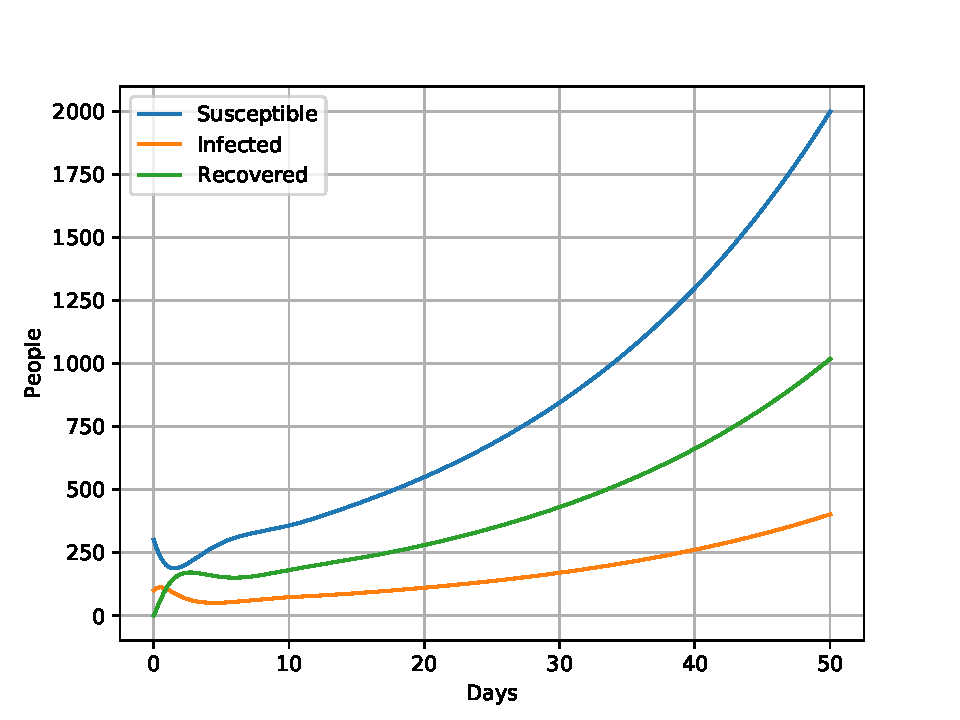
\includegraphics[scale=0.56]{../plots/opp_c_h_100000.pdf} %denne?
	\caption{Plots of popualtion $B$  when accounting for vital dynamics with $d_i=0.1$, and $d$ and $e$ is increased by a factor of 1000, 2000 and 10000 respectively.}
	%Label gjør det enkelt å referere til ulike bilder.
	\label{opp_c2}
\end{figure}


\subsection{Seasonal Variation}

\begin{figure}[!htb]
	\centering 
	%Scale angir størrelsen på bildet. Bildefilen må ligge i samme mappe som tex-filen. 
	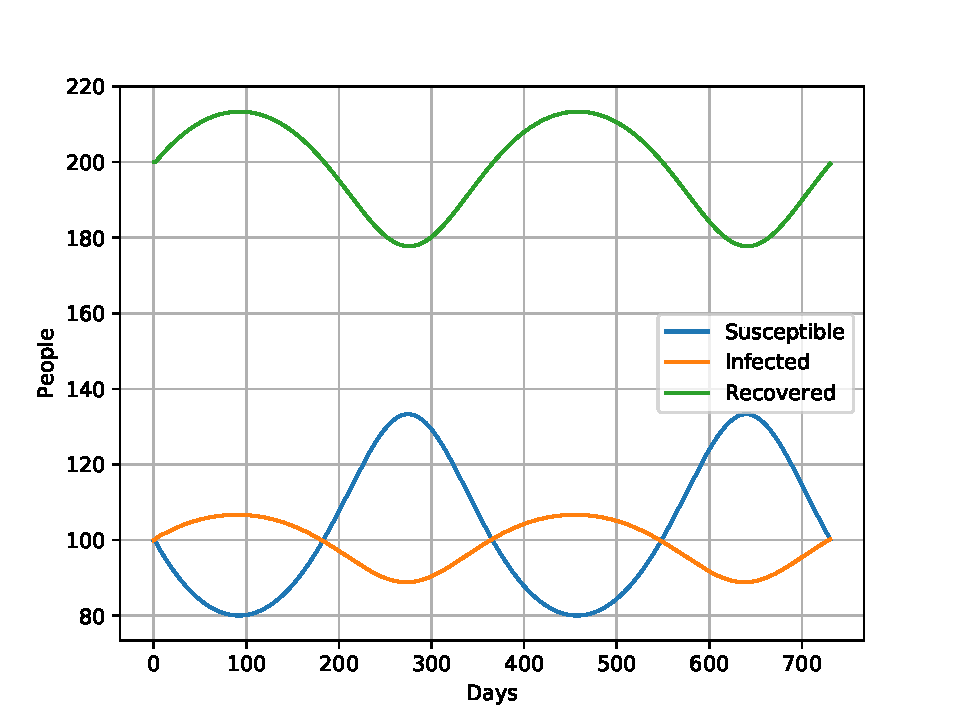
\includegraphics[scale=0.56]{../plots/opp_d_A.pdf}
	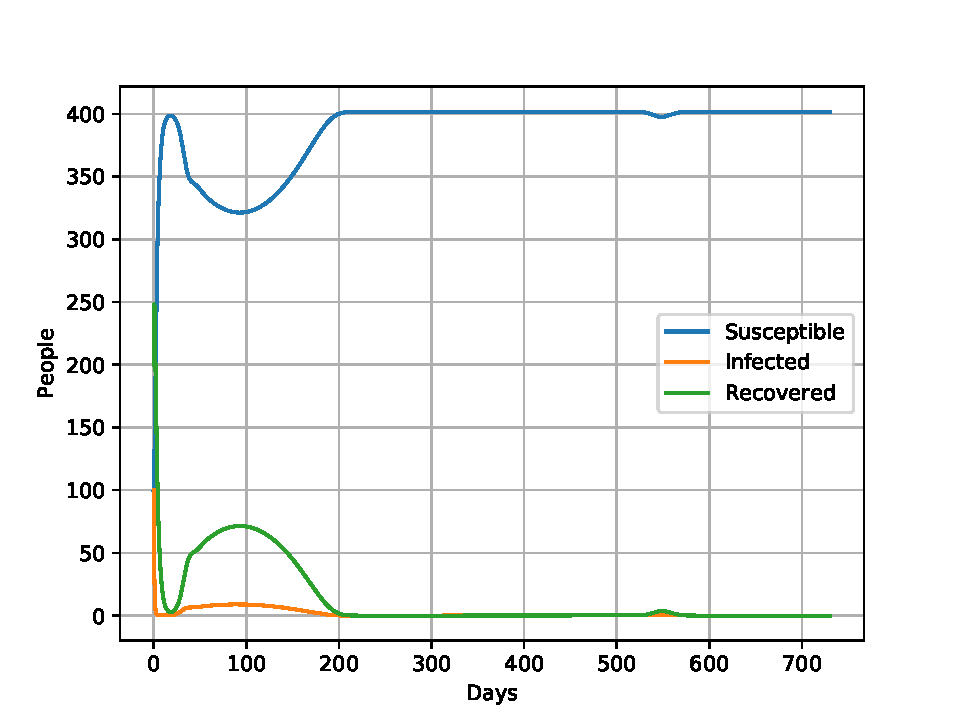
\includegraphics[scale=0.56]{../plots/opp_d_B.pdf}
	\caption{Plots of population $A$ in the left and $D$ on the rigth when $a$ varies with time. $A=1$ and $a0=4$.}
	%Label gjør det enkelt å referere til ulike bilder.
	\label{opp_d0}
\end{figure}
\begin{figure}[!htb]
	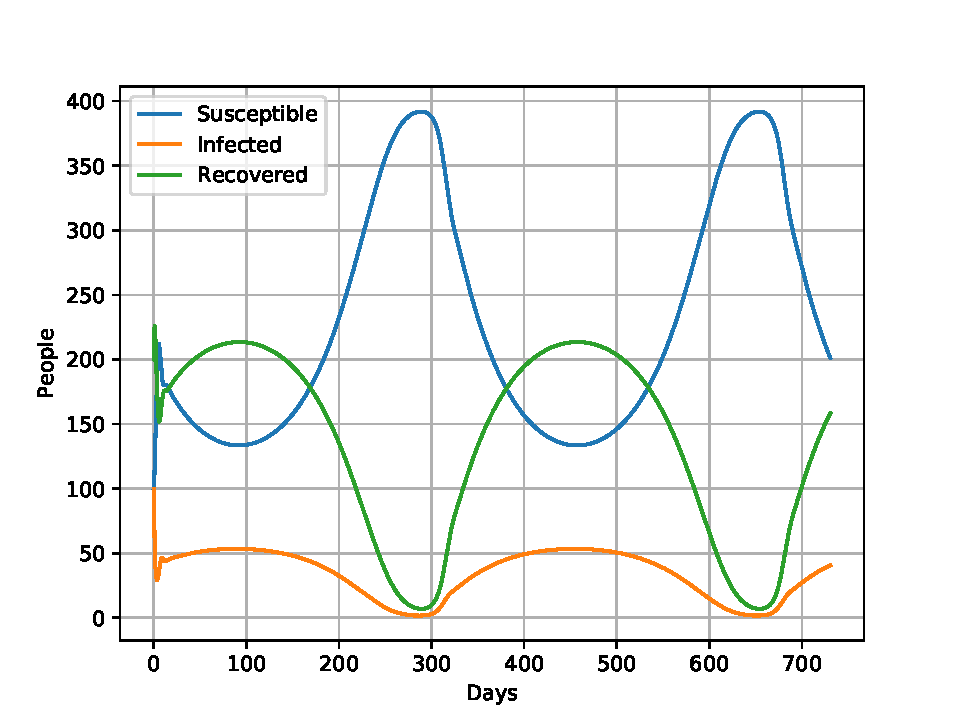
\includegraphics[scale=0.56]{../plots/opp_d_C.pdf}
	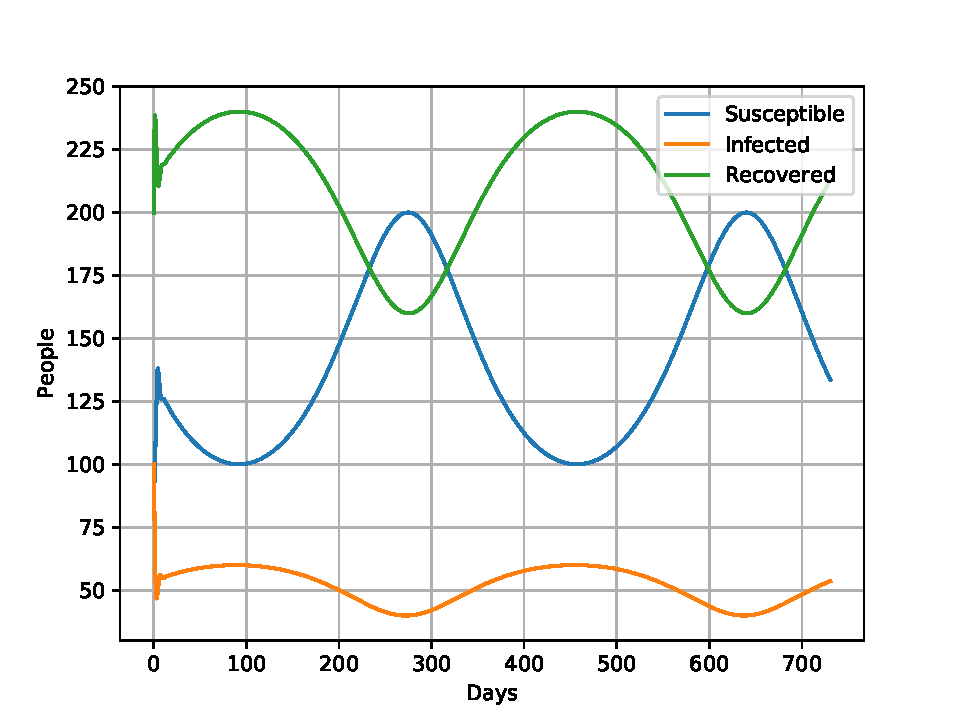
\includegraphics[scale=0.56]{../plots/opp_d_D.pdf}
	\caption{Plots of population $B$ when $a$ varies with time. $A=2$, while $a0=4$ on the left and $a0=6$ on the rigth.}
	%Label gjør det enkelt å referere til ulike bilder.
	\label{opp_d1}
\end{figure}


\subsection{Vaccination}

\begin{figure}[!htb]
	\centering 
	%Scale angir størrelsen på bildet. Bildefilen må ligge i samme mappe som tex-filen. 
	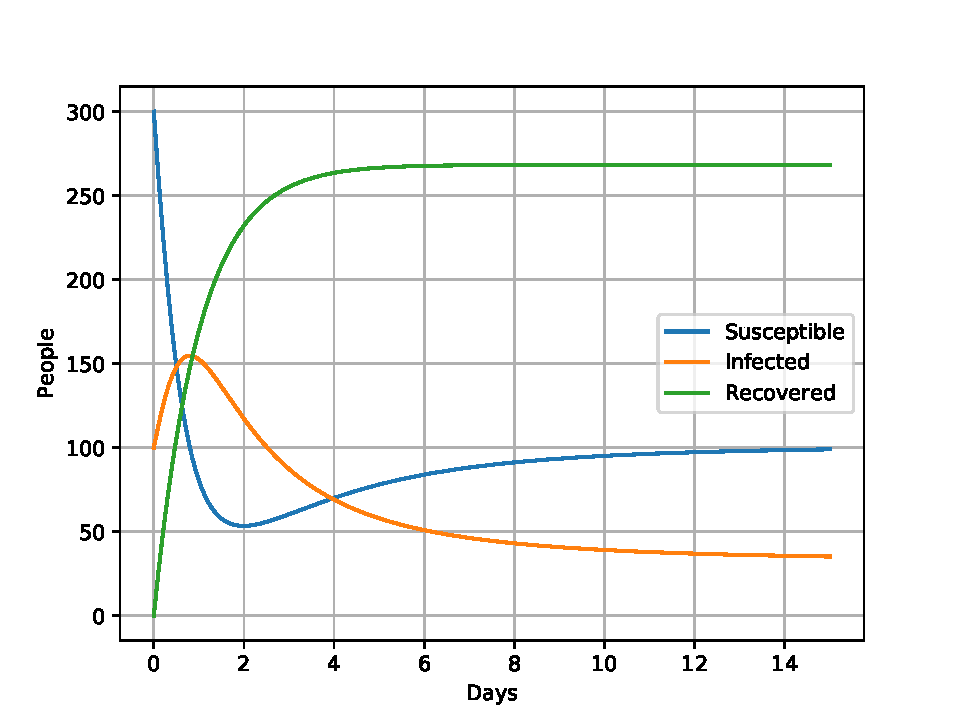
\includegraphics[scale=0.56]{../plots/opp_e_A0.pdf}
	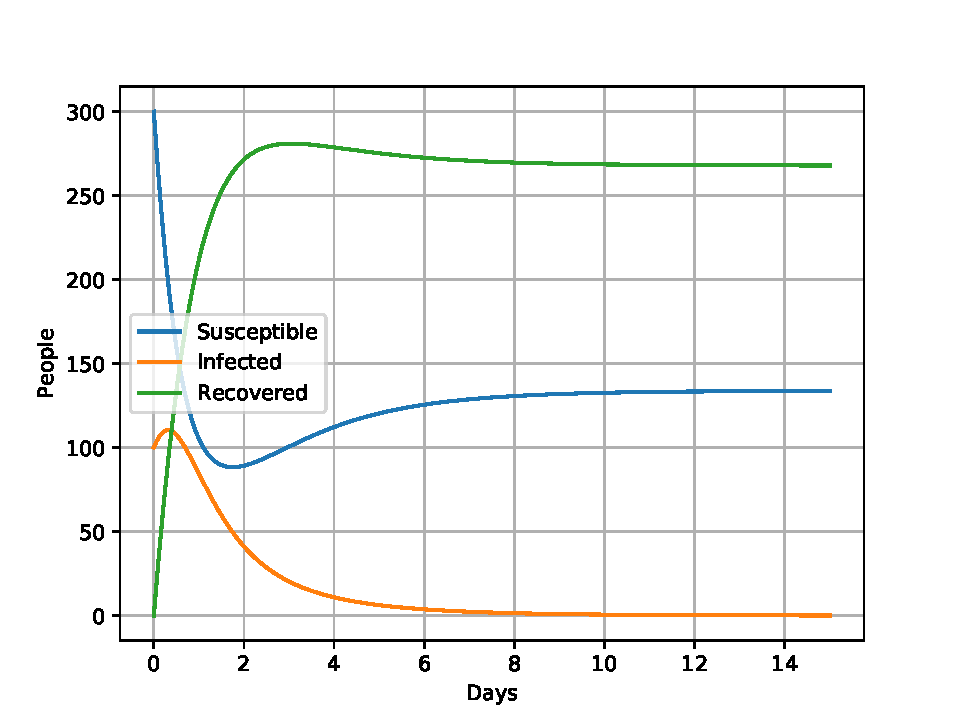
\includegraphics[scale=0.56]{../plots/opp_e_B0.pdf}	
	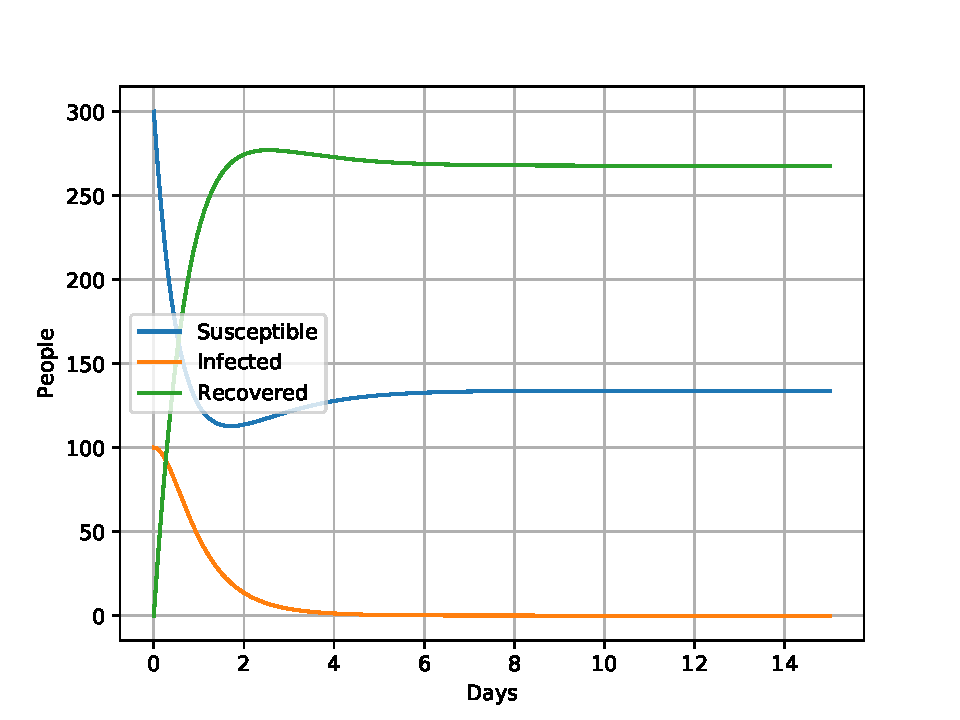
\includegraphics[scale=0.56]{../plots/opp_e_C0.pdf}
	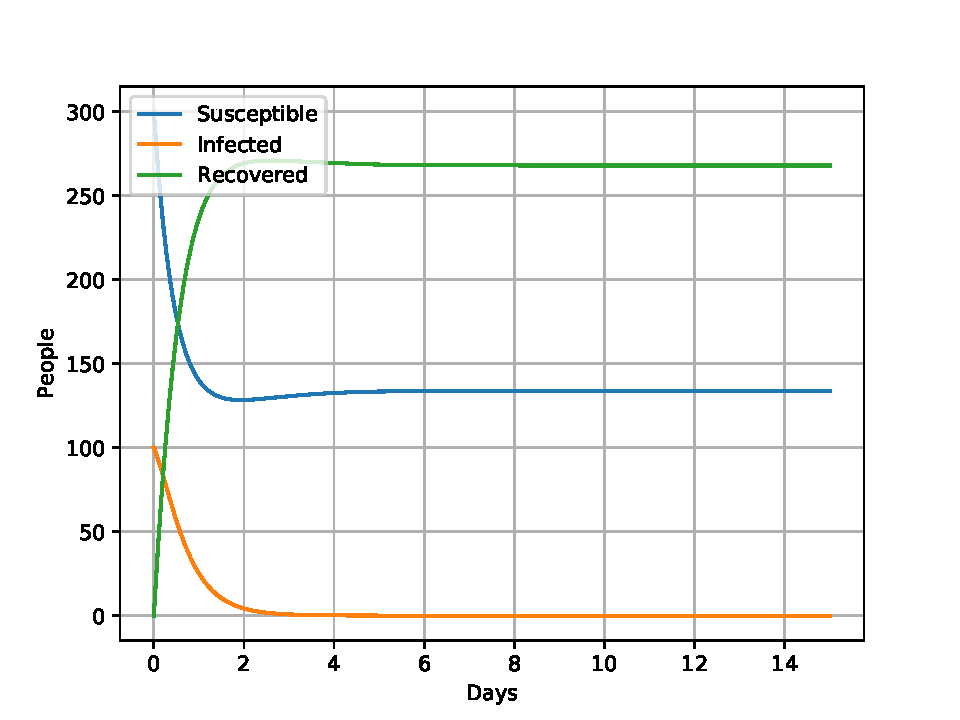
\includegraphics[scale=0.56]{../plots/opp_e_D0.pdf}
	\caption{Plots of population $A$ to $D$ with constant vaccination $f=1$.}
	%Label gjør det enkelt å referere til ulike bilder.
	\label{opp_e0}
\end{figure}

\begin{figure}[!htb]
	\centering 
	%Scale angir størrelsen på bildet. Bildefilen må ligge i samme mappe som tex-filen. 
%	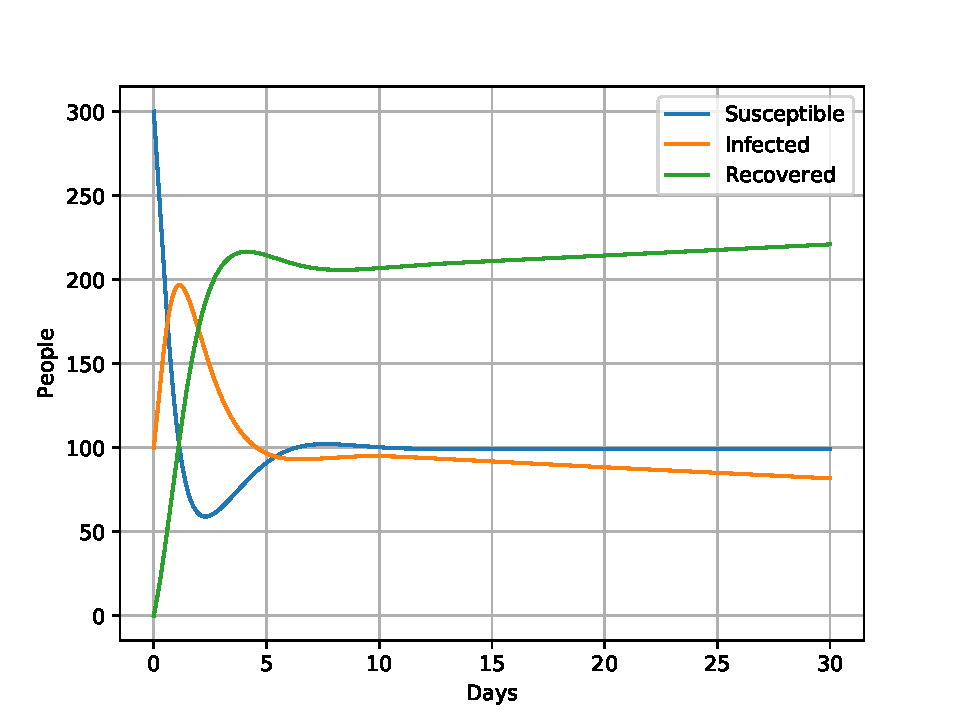
\includegraphics[scale=0.56]{../plots/opp_e_A1.pdf}
	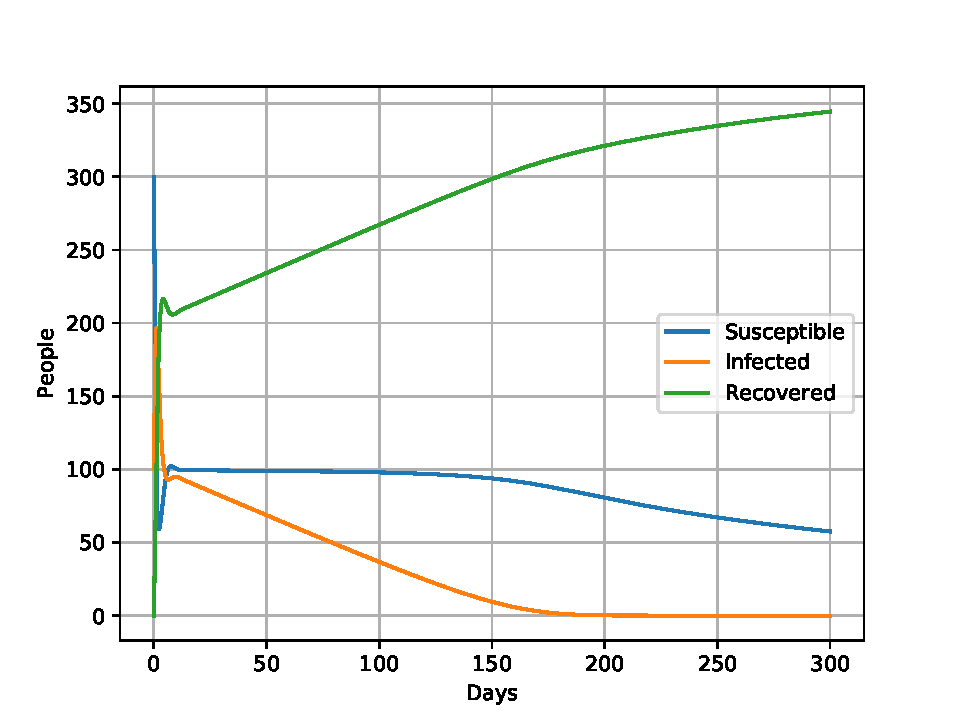
\includegraphics[scale=0.56]{../plots/opp_e_A2.pdf}
%	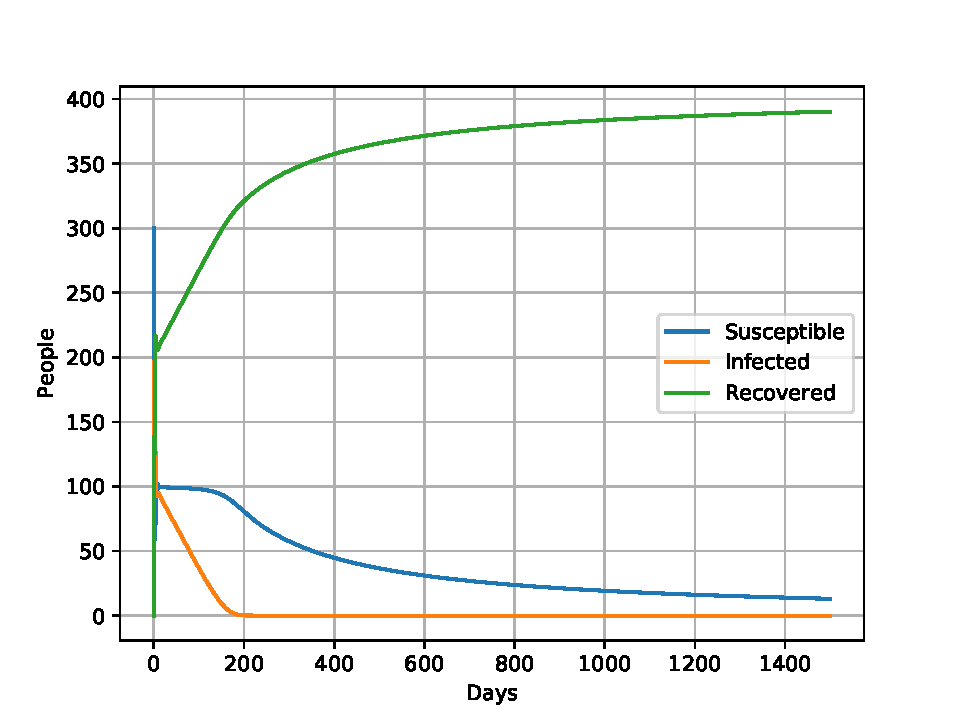
\includegraphics[scale=0.56]{../plots/opp_e_A3.pdf}
%	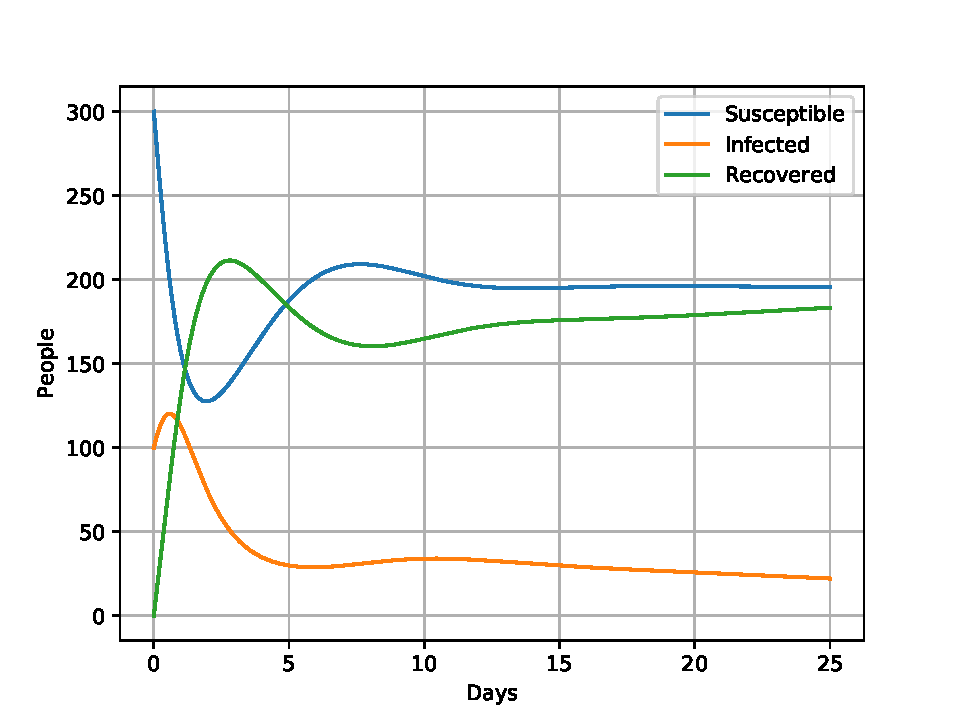
\includegraphics[scale=0.56]{../plots/opp_e_B1.pdf}	
	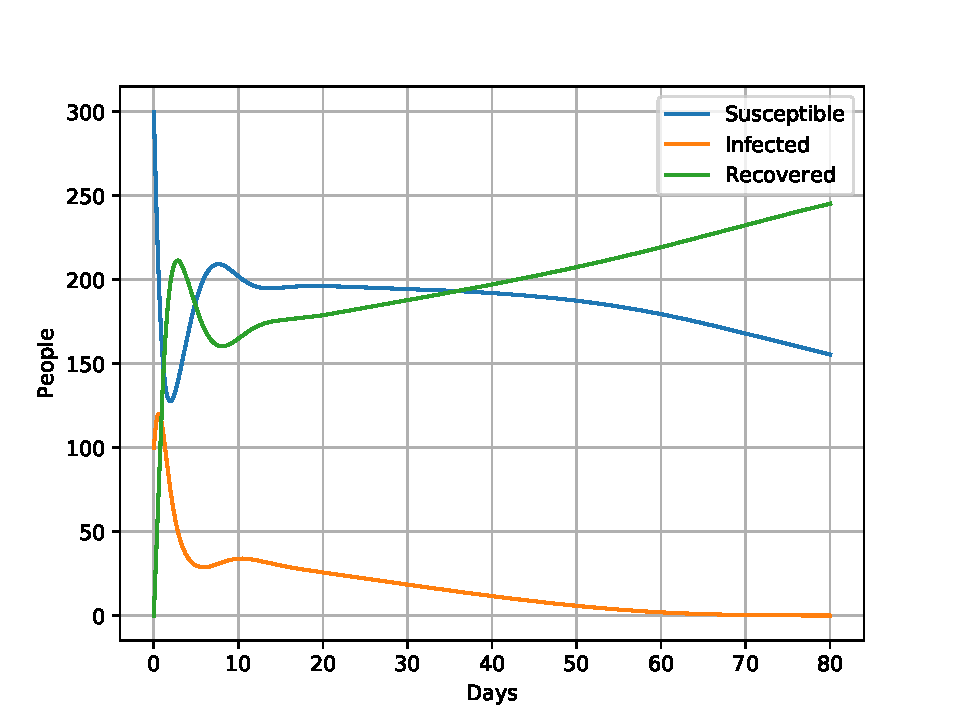
\includegraphics[scale=0.56]{../plots/opp_e_B2.pdf}	
%	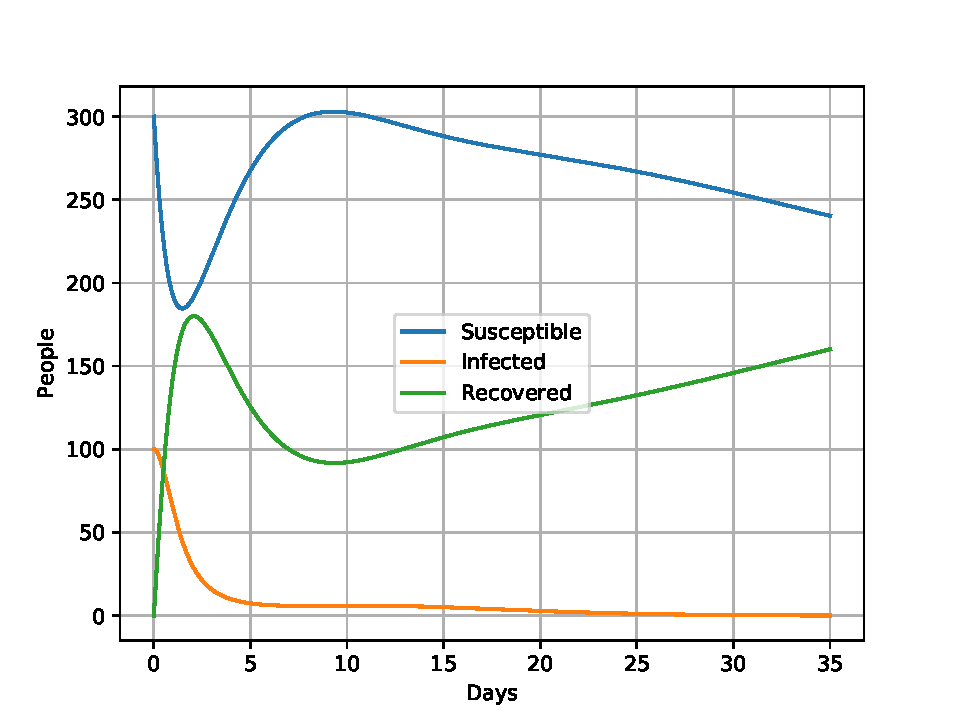
\includegraphics[scale=0.56]{../plots/opp_e_C1.pdf}
	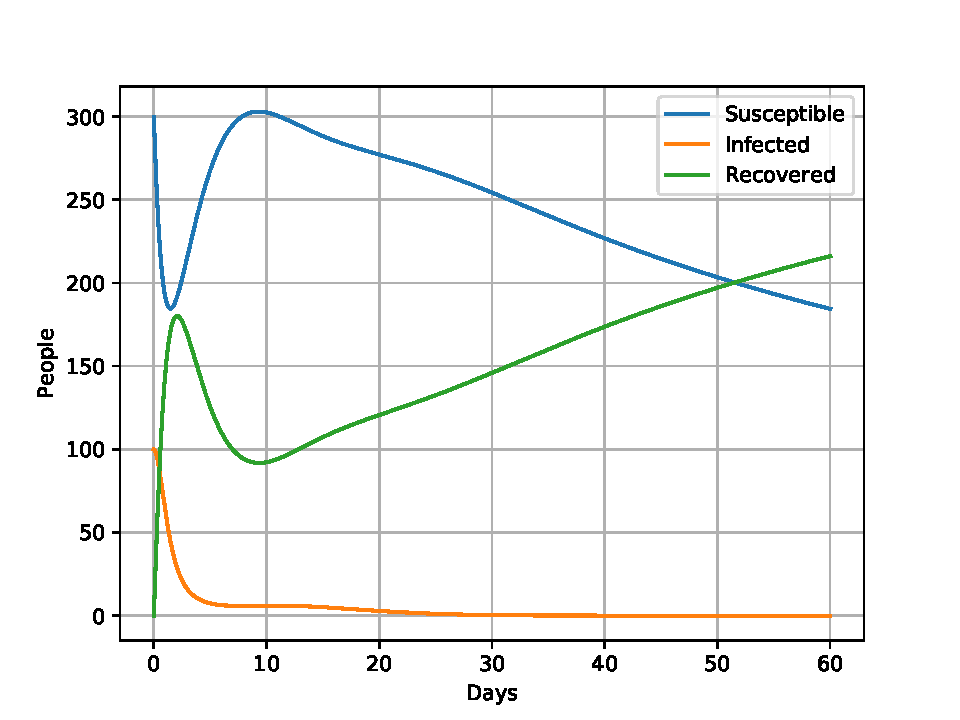
\includegraphics[scale=0.56]{../plots/opp_e_C2.pdf}
%	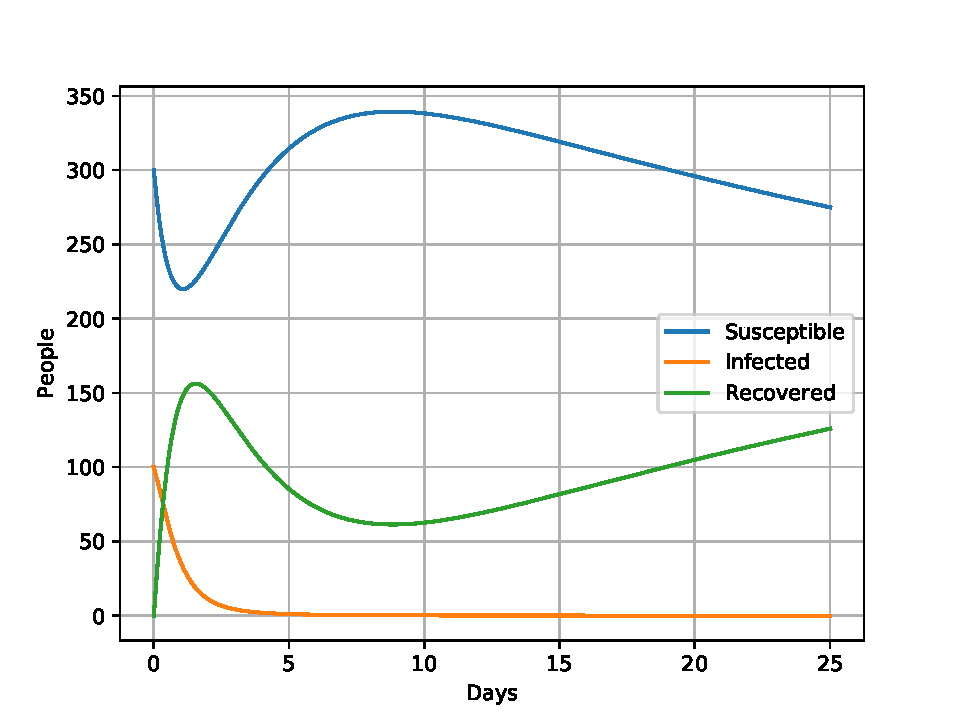
\includegraphics[scale=0.56]{../plots/opp_e_D1.pdf}
	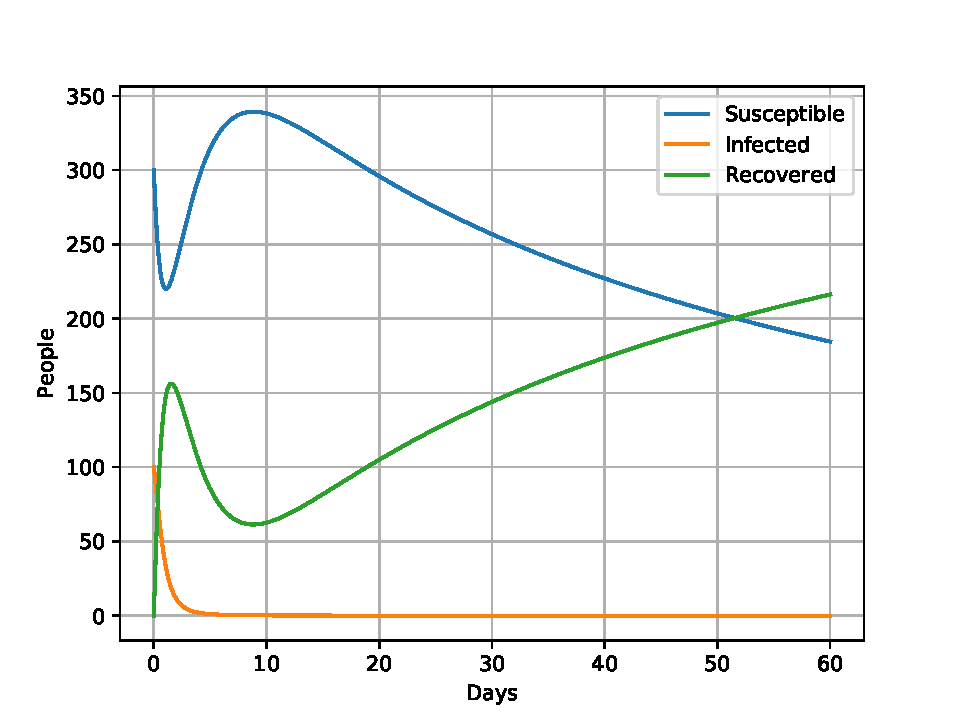
\includegraphics[scale=0.56]{../plots/opp_e_D2.pdf}
	\caption{Plots of population $A$ to $D$ with linear vaccination $f=0.1 t$.}
	%Label gjør det enkelt å referere til ulike bilder.
	\label{opp_e1}
\end{figure}

\begin{figure}[!htb]
	\centering 
	%Scale angir størrelsen på bildet. Bildefilen må ligge i samme mappe som tex-filen. 
	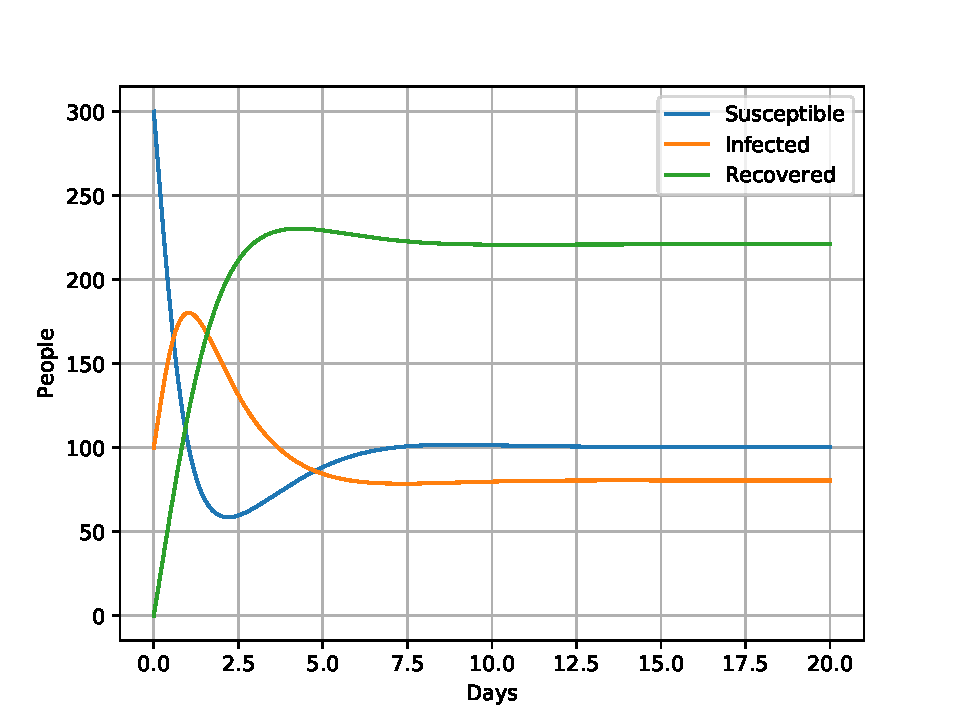
\includegraphics[scale=0.56]{../plots/opp_e_fa.pdf}
	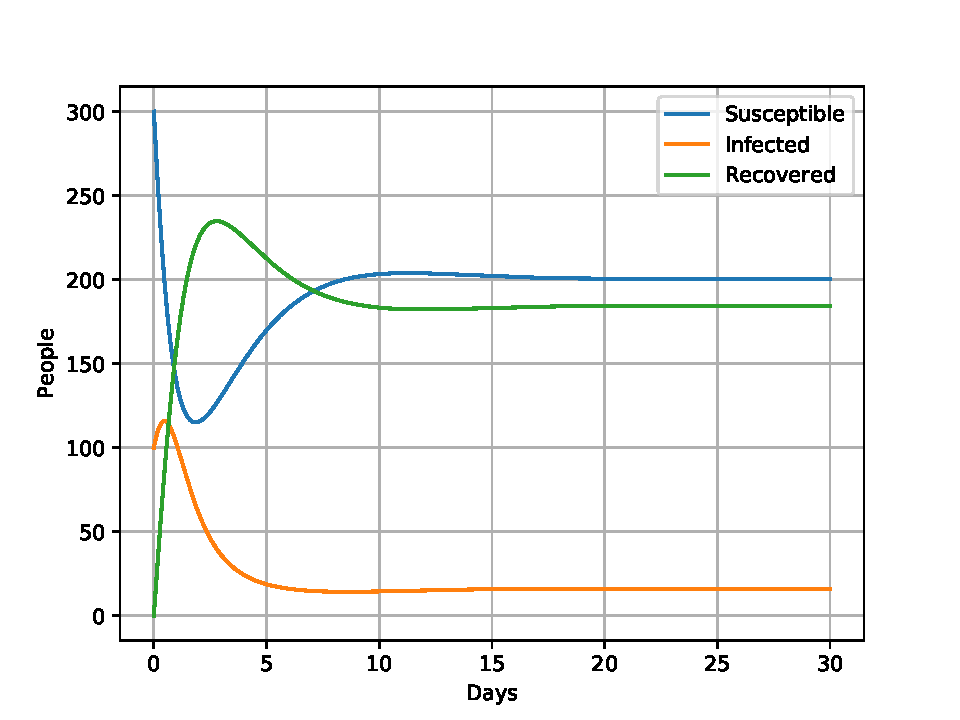
\includegraphics[scale=0.56]{../plots/opp_e_fb.pdf}	
	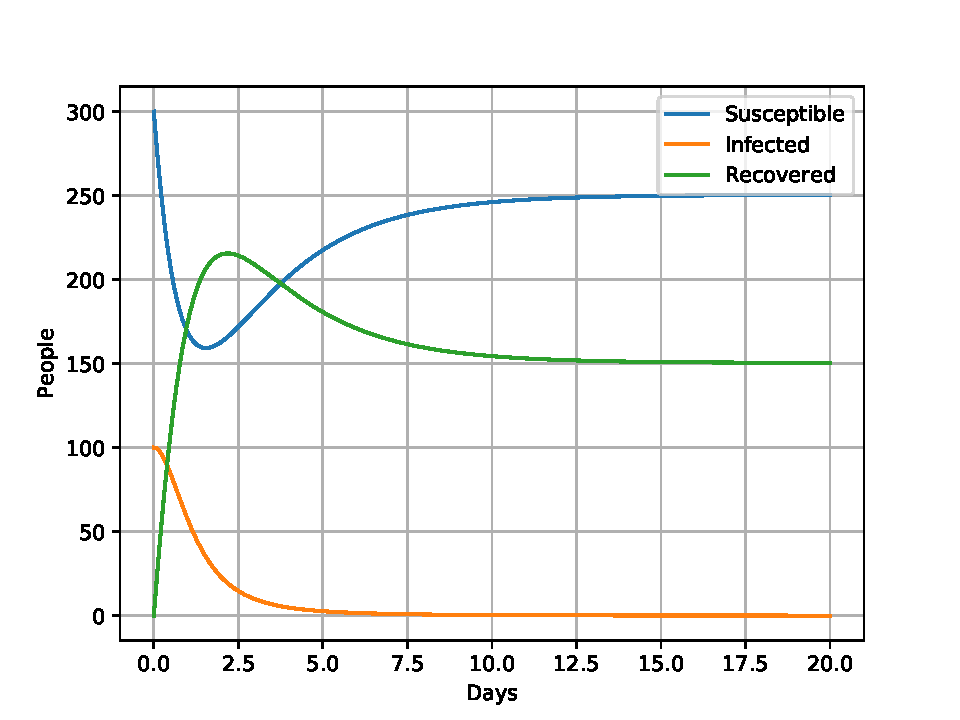
\includegraphics[scale=0.56]{../plots/opp_e_fc.pdf}
	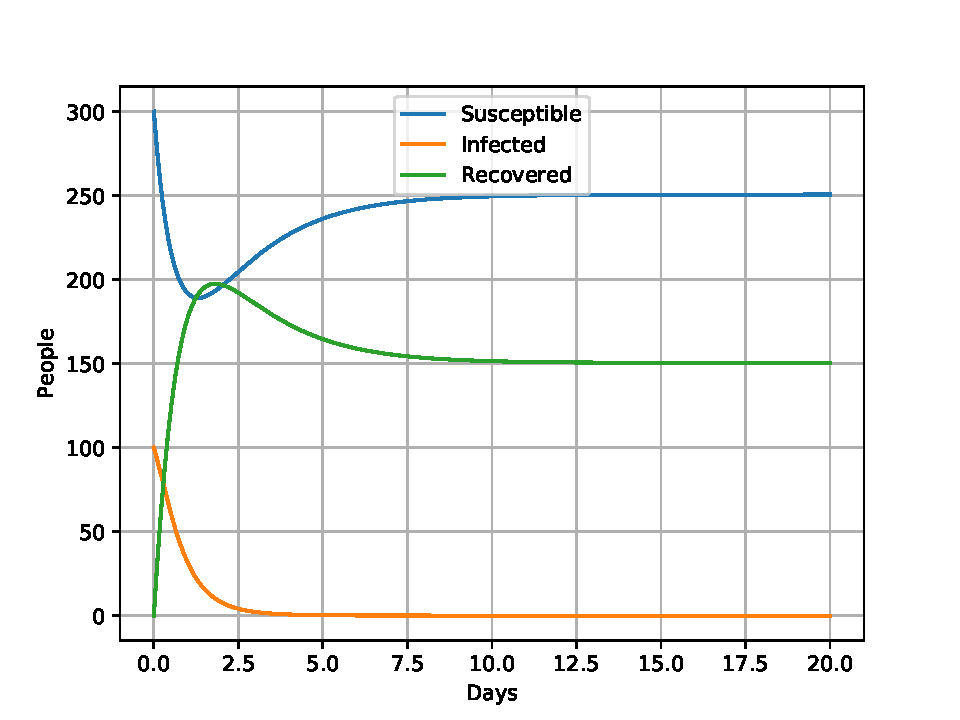
\includegraphics[scale=0.56]{../plots/opp_e_fd.pdf}
	\caption{Plots of population $A$ to $D$ with a vaccination campaign from day 2 to 9, where $f=0.3$, while it's 0 the rest of the time.}
	%Label gjør det enkelt å referere til ulike bilder.
	\label{opp_e2}
\end{figure}



\section{DISCUSSION}



\section{CONCLUTION}




%\newpage
\section{APPENDICES}
All the calculations were done using the programing language Julia. The programs used can be found at:
\url{}.
	
%\section{REFERENCES}
\begin{thebibliography}{9}
	\bibitem{lecture notes}
	Computational Physics, Lecture Notes Fall 2015, Morten Hjort-Jensen p. 419-424
\end{thebibliography}




%\begin{figure}[h!]
%	\centering 
%	%Scale angir størrelsen på bildet. Bildefilen må ligge i samme mappe som tex-filen. 
%	\includegraphics[scale=0.7]{opp2_7.pdf}
%	\caption{A plot of the entropy}
%	%Label gjør det enkelt å referere til ulike bilder.
%	\label{2.7}
%\end{figure}







	
	
	
	
	
	
	
	
	
	
	
	
	
	
	
\end{document}




